% Springer Nature LaTeX template, December 2024 release.
% Prepared for a Research Article in BMC Biomedical Engineering.
\documentclass[referee,lineno,pdflatex,sn-vancouver-num]{sn-jnl}

\usepackage{graphicx}
\usepackage{amsmath,amssymb}
\usepackage{booktabs}
\usepackage{multirow}
\usepackage{xurl}
\usepackage{placeins}
\graphicspath{{./}}
\raggedbottom

\begin{document}

\title[Physics-based evaluation of prosthetic regression]{Towards the Use of Simulated Environments to Evaluate sEMG-Based Prosthetic Knee-Angle Regression}

\author*[1]{\fnm{Aaron} \sur{Xiong}}
\affil*[1]{\orgname{Independent researcher}, \country{United States}}

\abstract{\textbf{Background:} Knee-angle regression models are normally evaluated with root mean squared error (RMSE). RMSE shows how closely a prediction follows a recorded knee trajectory, but it does not show whether the prediction preserves whole-body walking behavior. This study tested whether a confirmed sEMG improvement in 100-ms knee-angle prediction also reduced instability in a physics-based walking simulation.

\textbf{Results:} A participant-calibrated residual-fusion model was developed with 30 participants from the public Gait120 dataset and evaluated once in 90 separate participants. Eighty one-second level-walking windows were matched to MoCapAct humanoid references, and the paired prediction errors were inserted into the same matched MuJoCo motions. Adding sEMG reduced mean participant RMSE from 5.093$^{\circ}$ to 4.748$^{\circ}$ (mean improvement 0.345$^{\circ}$, 95\% confidence interval 0.252--0.438$^{\circ}$; paired $t(89)=7.39$, $p=7.50\times10^{-11}$); 70 of 90 participants improved. Mean motion-matching errors were 4.317$^{\circ}$ for the knee and 3.630$^{\circ}$ for right-thigh pitch. The mean reduction in excess-instability area under the curve was $-0.0012$ score-seconds (95\% confidence interval $-0.0105$ to 0.0081; paired $t(64)=-0.25$, $p=0.801$). After knee and thigh matching errors were accounted for, RMSE was not associated with excess instability (partial Spearman $\rho=-0.145$, 95\% confidence interval $-0.370$ to 0.082; $p=0.248$). Across seven fixed training-data fractions, the directly observed physical deterioration occurred between the 13.41$^{\circ}$ and 16.29$^{\circ}$ RMSE checkpoints, where balance losses increased from 3 to 32 of 80 windows.

\textbf{Conclusions:} sEMG produced a small and repeatable improvement in 100-ms knee-angle prediction, but this improvement did not reduce simulated whole-body instability. Very poor prediction did destabilize walking, indicating that physical simulation can distinguish errors that are not separated by the final model's narrow RMSE range.}

\keywords{surface electromyography, knee-angle prediction, prosthetic control, biomechanics, MuJoCo, motion matching, extrapolated center of mass}

\maketitle

\section{Introduction}\label{sec:introduction}

Lower-limb amputation remains a substantial rehabilitation problem in the United States, and transfemoral (above-the-knee) amputation is especially disruptive because it removes the knee joint and many of the mechanical advantages that it provides during standing, walking, sitting, and transitions onto different terrain \cite{dillingham2002}. Even with contemporary microprocessor-based artificial knees, users frequently walk more slowly, expend more mechanical work, and experience functional limitations that can vary from one wearer to another \cite{pinhey2022}. Following from these limitations of the status quo, the main goal of current research continues to be the accurate reconstruction of the knee trajectory across changing gait states, variable sensor conditions, and differences in movement and body structure from patient to patient.

The major challenge in transfemoral prosthetics is that direct information about the missing or mechanically replaced knee is unavailable to predictive solutions for the knee angle. A reconstructive algorithm must instead infer knee behavior from nearby available signals that are practical and preferably non-invasive to collect from the patient. Surface electromyography (sEMG) provides a window into muscle activations, while recorded kinematics describe the motion that has already occurred \cite{deluca1997,farina2014}. These signals are valuable for different reasons. sEMG contains neuromuscular information, but is noisy, non-stationary, and sensitive to fatigue, variation in electrode placement, skin impedance, and inter-subject variability, which is why machine-learning techniques are commonly used to process this volatile signal \cite{chowdhury2013,phinyomark2018}. Kinematic history is comparatively stable, but does not directly measure muscle activation that precedes the resulting movement. The task of prediction, or regression, as it is referred to in the literature, involves combining the sEMG signal with contextual kinematic data to estimate the knee angle at a future horizon.

\subsection{Current Methods for Knee-Angle Prediction}

This major inference problem has been studied with both classical and deep methods in machine learning. Earlier work in myoelectric control relied heavily on feature-engineered models and pattern-recognition pipelines, while more recent studies have used convolutional, recurrent, and transformer-based models to estimate continuous lower-limb motion \cite{hargrove2007,sun2022,yi2022}. Sun et al. combined kinematic and myoelectric signals for continuous knee-angle estimation, and Yi et al. used both inputs to predict lower-limb kinematics \cite{sun2022,yi2022}. At the same time, systematic reviews of EMG-driven lower-limb prosthetic control still describe the field as methodologically evolving, particularly with respect to preprocessing, participant calibration, validation strategy, and model architecture \cite{cimolato2022,ahkami2023}.

The present study did not attempt to create another complex neural-network architecture. Its purpose was to preserve the physics-based evaluation from the original paper while replacing the former CNN--BiLSTM predictor, whose sEMG ablation had not improved prediction. A participant-calibrated residual-fusion model was therefore used so that the contribution of sEMG could be tested directly. The model first predicted the future knee angle from recorded knee history and then used sEMG to estimate the remaining error. Removing sEMG only removed this correction; every other part of the predictor remained the same.

The forecast horizon also changes the meaning of the task. Estimating the present knee angle does not provide time for prosthetic actuation, whereas an ahead-of-time prediction can do so. Coker et al. examined 50-, 100-, 150-, and 200-ms knee forecasts, and Yi et al. reported a useful ahead-of-time interval of approximately 27--108 ms \cite{coker2021,yi2022}. The electromechanical delay between muscle activity and measurable force provides an additional physiological reason to examine sEMG before the resulting motion \cite{cavanagh1979}. A 100-ms horizon was selected before model development because it was directly tested in prior knee-prediction research, lies within the interval reported by Yi et al., and provides a more meaningful lead time than the 10-ms horizon in the previous version of this study.

\subsection{Simulation of Virtual Prosthetics}

The primary problem with the current evaluation metric, cross-validation RMSE, is that prediction accuracy alone does not guarantee the prosthetic's true usefulness in an actual kinematic context. Joint-angle regressors are only valuable if their outputs are biomechanically plausible when considered in the context of whole-body motion. This gap between statistical error and real-time function has already been examined in myoelectric control research. Hargrove et al., for example, evaluated a pattern-recognition controller through a real-time virtual environment rather than solely reporting classifier accuracy \cite{hargrove2007}. Similarly, Krasoulis et al. showed that prosthetic finger performance improved with user practice and could not be reliably inferred from machine-learning statistics alone \cite{krasoulis2019}. Together, these studies suggest that a low RMSE could hide functionally poor control of the prosthetic.

Another issue is that real human-subject testing is difficult, expensive, and potentially risky. Testing a weak or unstable controller on an actual prosthesis could create safety concerns for the user. For that reason, virtual environments and physics-based simulation can serve as an intermediate evaluation layer between offline prediction and real-world trials.

Physics-based simulation offers a closer approximation to a real-life locomotion context because it models bodies using joints, forces, contacts, and dynamics instead of simply displaying a motion visually. One implementation of physics-based simulation is MuJoCo, a physics engine commonly used in research for model-based control and simulated articulated bodies \cite{todorov2012}. For prosthetic research, this kind of engine is valuable because it can test whether a predicted movement is dynamically plausible in a controlled environment. A simulated body can fall, lose balance, or react poorly to a control signal, which provides information that a static prediction-error number cannot provide.

Motion-capture-based resources also help make simulation more realistic. MoCapAct provides motion-capture-based humanoid control data, allowing simulated movement to be grounded in recorded human-like motion rather than arbitrary synthetic poses \cite{wagener2022}. One derivative technique is motion matching, a related idea from video-game character animation in which a system searches a database for the motion clip that best matches a query \cite{clavet2016}. In a prosthetic-evaluation context, motion matching is useful because it can place a predicted joint trajectory into a broader whole-body movement context. Without that context, a knee prediction remains only a time-series output; with context, it can be examined as part of a simulated gait sequence.

It is important to note that simulation is not a replacement for real human testing. A simulated body is still a simplified model of a real person, and simulated instability is not the same as a clinical fall outcome. However, simulation can still expose a gap between local prediction accuracy and whole-body functional behavior. A model that performs well by RMSE may produce a trajectory that is poorly timed, physically awkward, or destabilizing once inserted into a locomotion system. Conversely, a slightly higher-RMSE trajectory may not be physically harmful if its errors occur in less sensitive parts of the gait cycle. By opening the door for investigation into the ability of RMSE to predict functional performance, simulation helps test whether numerical prediction metrics represent real practical ability in a prosthetic algorithm.

\subsection{Balance Metrics and Functional Evaluation}

A common method of physically evaluating locomotion behavior is to evaluate the balance of a full-body system during a walk cycle. This is traditionally done by finding the center of mass, or CoM, which constitutes the average concentration of the mass distributed across the body. During standing, keeping the CoM over the feet is closely related to staying balanced and upright. In a moving scenario, however, determining instability is more complex. A person's CoM may be in an acceptable position at one instant but still moving quickly enough that a corrective step is needed lest a loss of balance occur. The extrapolated center of mass, or XCoM, accounts for this by incorporating both the CoM and its velocity, allowing dynamic movement to be accounted for while examining balance \cite{hof2005,hof2008}.

To determine whether the XCoM is in an acceptable state, an area called the support polygon must be defined. In double support, or two-legged motion, the support polygon includes the area between both feet. The relationship between the XCoM and the support polygon is defined by a metric called the support margin; if the XCoM remains inside this margin near the support polygon, the body is generally easier to stabilize. If the XCoM strays too far, corrective steps by the legs may be necessary to prevent falling, resulting in high instability \cite{hof2005,hof2008}.

Functional evaluation in prosthetics research thus requires more than numerical predictive accuracy. Equally as, if not more important to consider is the question of whether or not the knee angle derived from the prediction model remains compatible with gait, support, and balance in a full physical context. The literature has made strong progress improving on current numerical benchmarks, but a remaining gap can be found by questioning whether those benchmarks are accurate representations of functional success. RMSE can show that a model reconstructs a target angle accurately, but it cannot by itself show whether that angle would preserve the balance and characteristics of the original motion as part of a physical system. This gap motivates simulation-based evaluation as the next step in the evaluation process of prosthetic regression models.

The present study addressed this gap through three questions. First, does sEMG reduce 100-ms knee-angle prediction error beyond the same kinematic model alone? Second, does that reduction lower instability when both predictions are tested in the same matched walking motion? Third, when the range of prediction error is deliberately widened, at what measured interval does the simulation begin to show a clear physical deterioration?

\section{Methodology}\label{sec:methodology}

\subsection{Data Preparation}

The prediction dataset was Gait120, a public resource containing synchronized kinematics and sEMG from 120 healthy adult male participants \cite{boo2025,boo2025dataset}. Only level walking was used. Stair walking, slope walking, sit-to-stand, stand-to-sit, and every other activity were excluded because the physical question in this paper concerns ordinary walking. The prediction data and the simulation reference library therefore represented the same general activity.

\begin{figure}[!htbp]
\centering
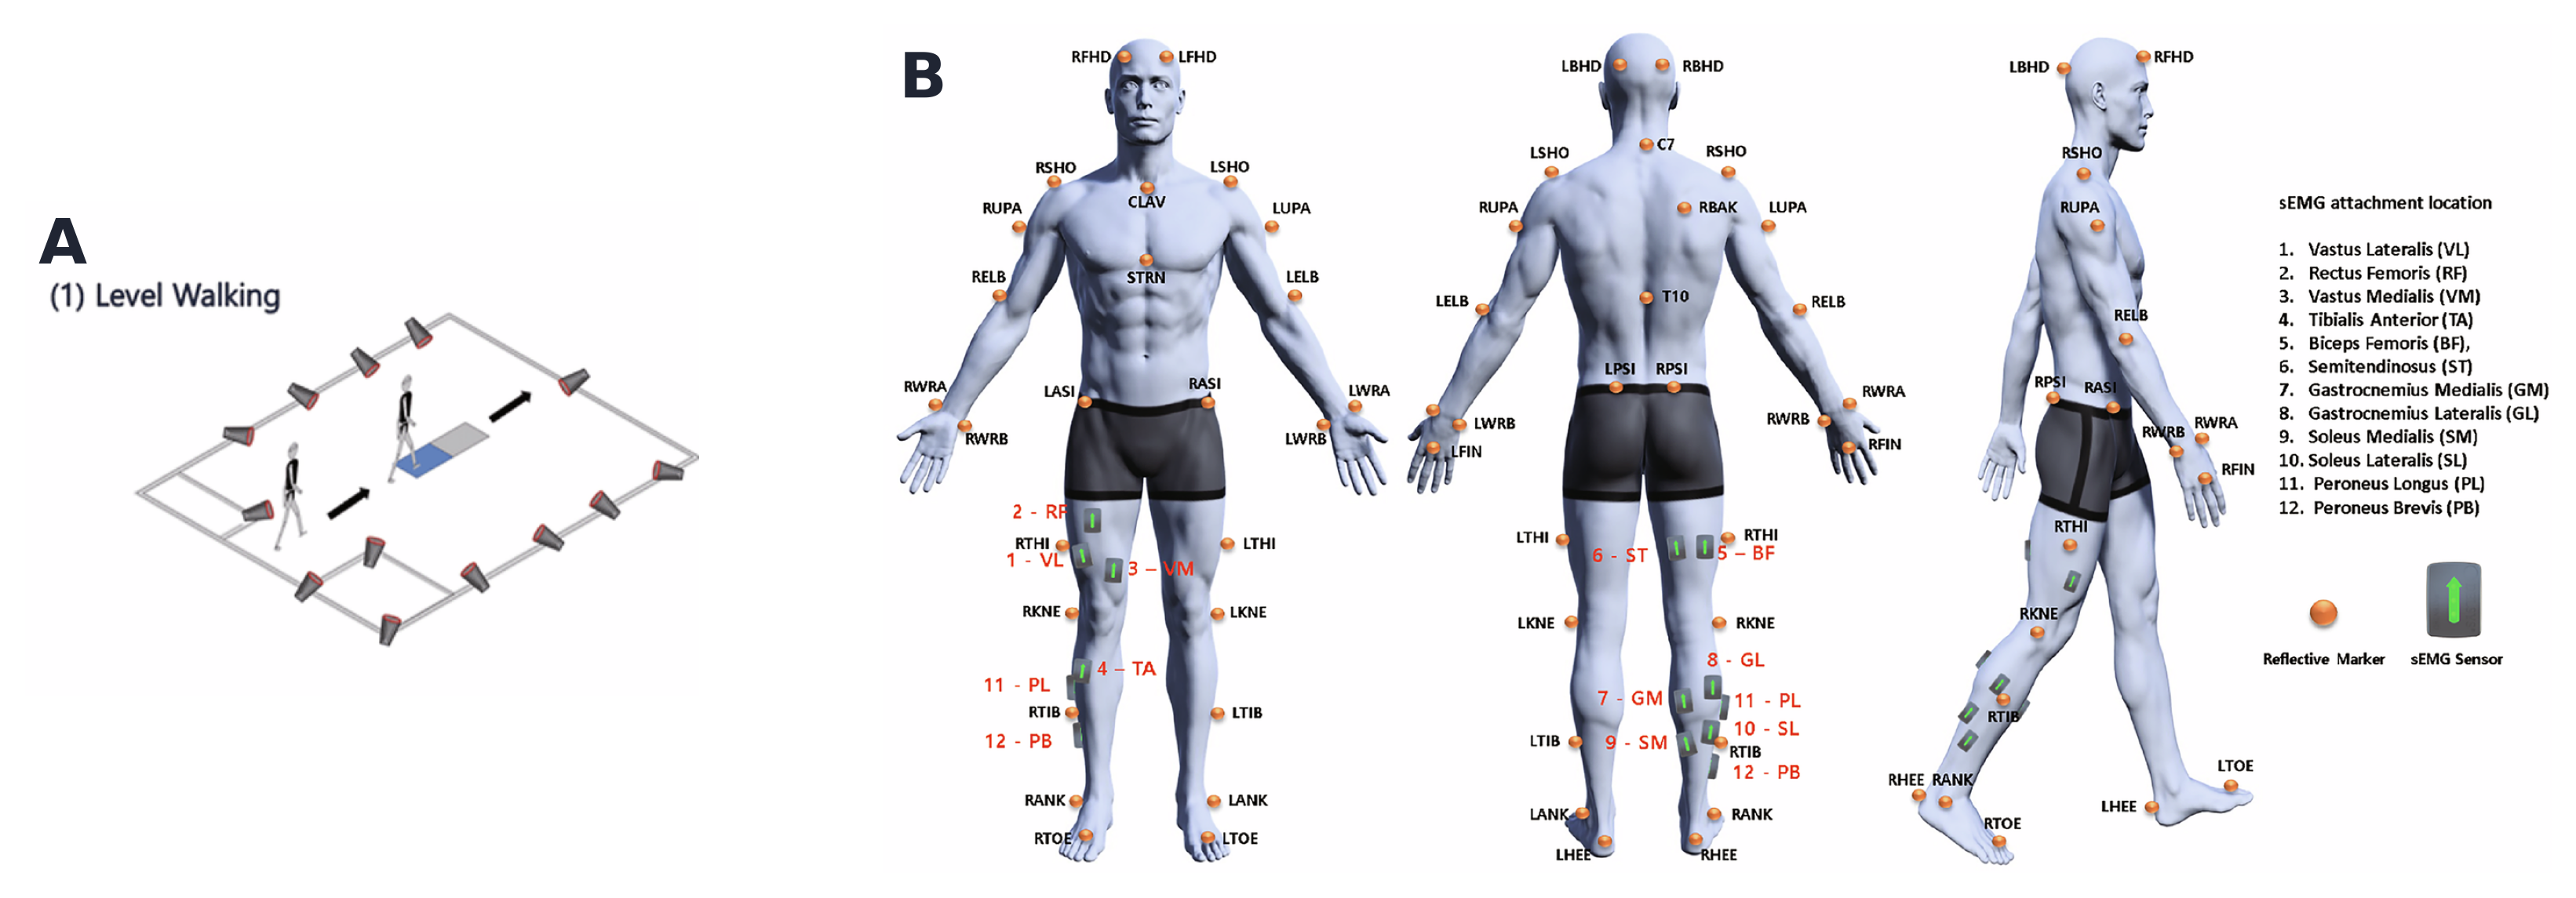
\includegraphics[width=0.88\textwidth]{gait120_data.png}
\caption{\textbf{Gait120 data collection.} Level-walking setup and lower-limb sEMG sensor locations, adapted from Boo et al. \cite{boo2025} under the Creative Commons Attribution 4.0 licence.}
\label{fig:gait120}
\end{figure}

\begin{figure}[!htbp]
\centering
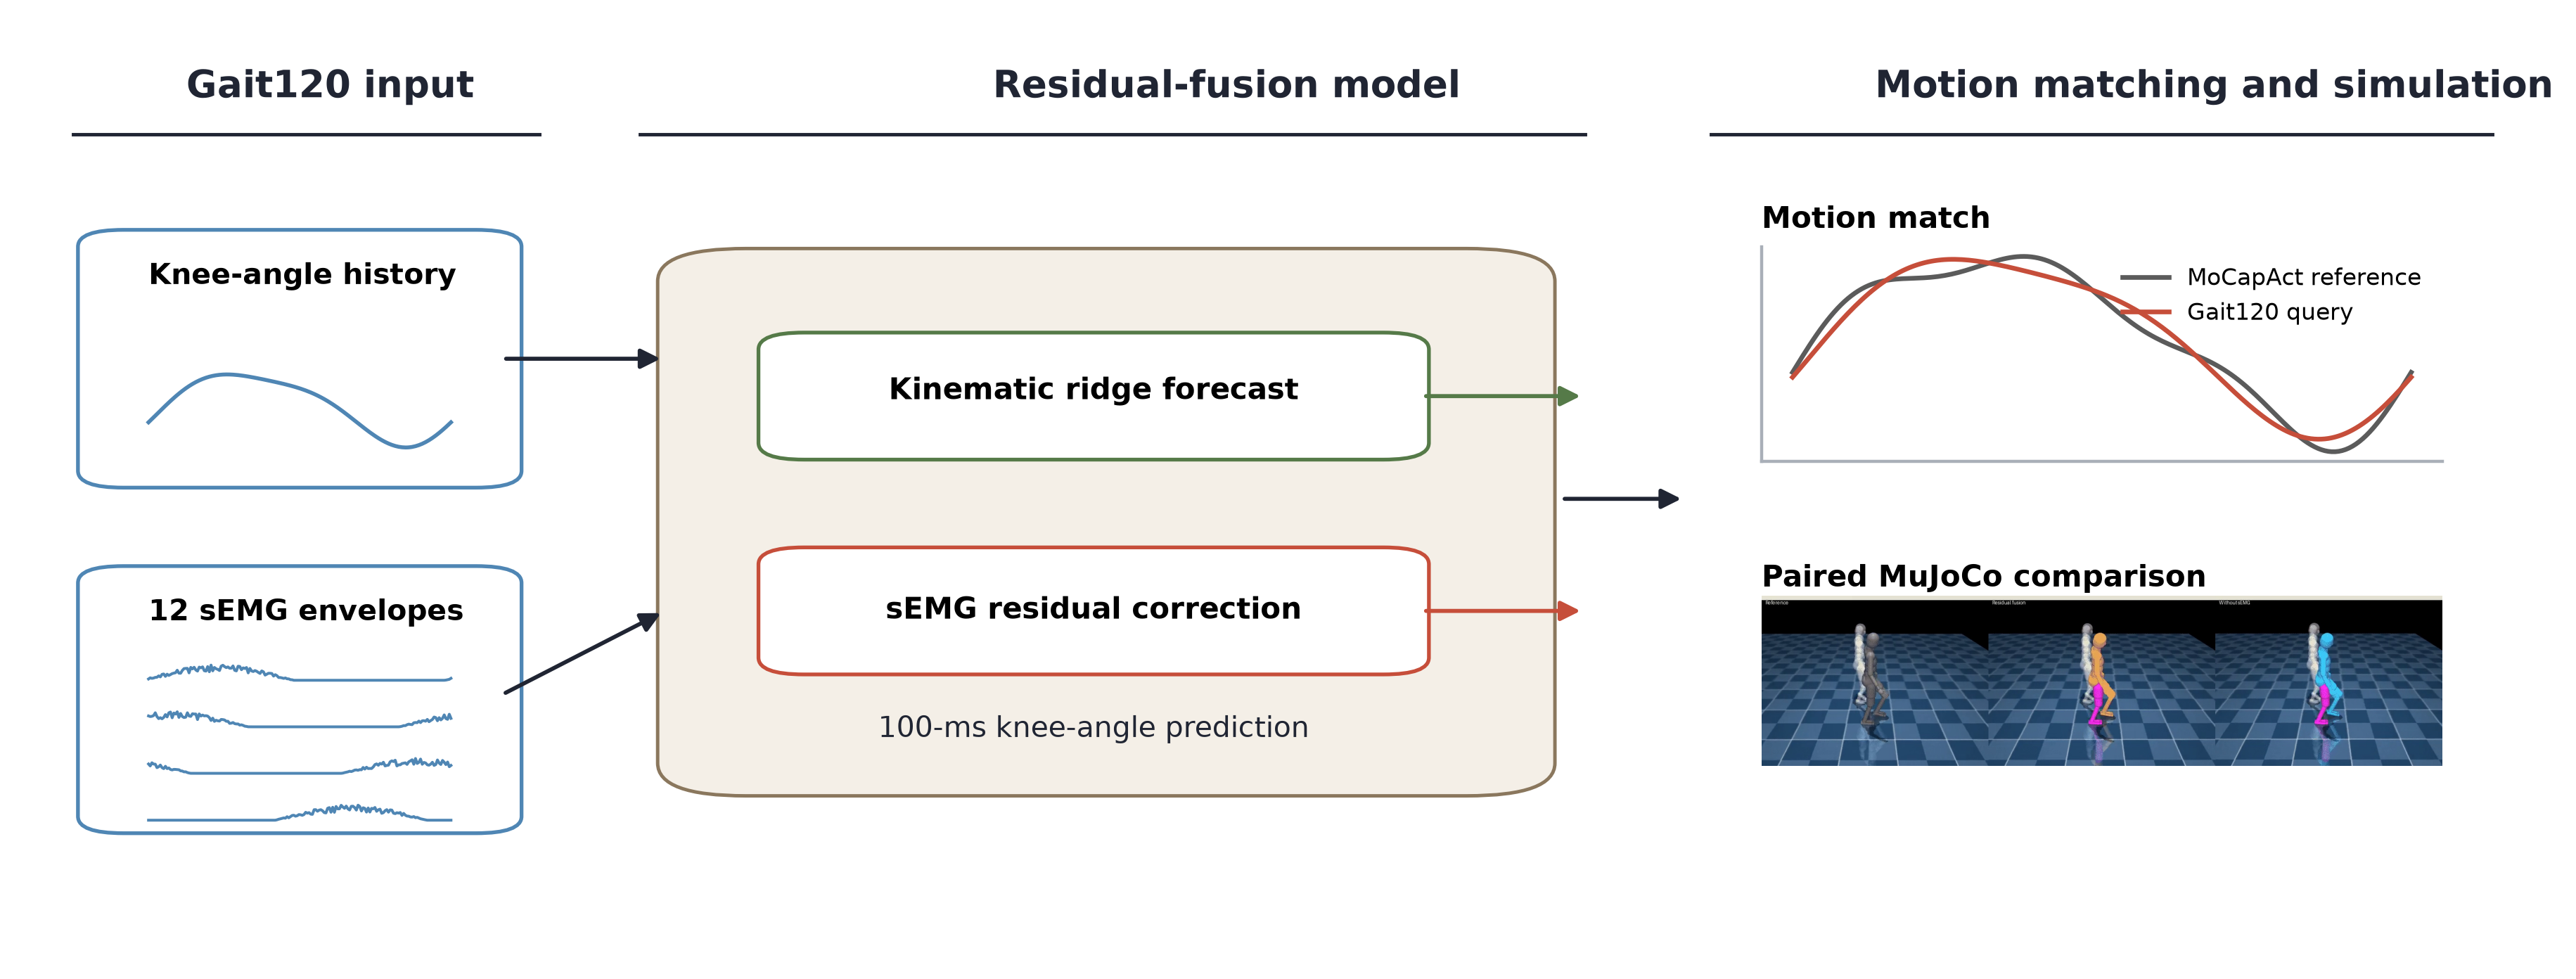
\includegraphics[width=\textwidth]{pipeline_overview.png}
\caption{\textbf{Study workflow.} The prediction, motion-matching, simulation, and statistical-analysis pipeline.}
\label{fig:pipeline}
\end{figure}

Participants S001--S030 formed the development group. Their first three trials were used to fit models, trial 4 was used to choose the two ridge penalties and residual weight, and trial 5 was used to check the selected model. In this paper, the development group is simply the group whose data were allowed to influence a model choice. Participants S031--S120 formed a separate confirmation group after the model inputs, penalties, residual weight, test conditions, and statistical requirements had been set. Their trials 1--3 were used to fit the same participant-calibrated model, trial 4 was reported without further model selection, and trial 5 was evaluated once. The participant, rather than an individual window, was the statistical unit. This separation prevents neighboring samples or repeated trials from the same participant from being treated as independent evidence \cite{roberts2017}.

No formal power calculation was used because the confirmation group consisted of all 90 participants not used during development. The analysis therefore reports the participant-level effects, their confidence interval, and the magnitude of the mean change rather than using sample size alone as evidence of an effect.

\subsection{Data Format}

The analysis read the released 2000-Hz raw sEMG and 100-Hz OpenSim joint-angle records. Twelve right-leg channels were used: vastus lateralis, rectus femoris, vastus medialis, tibialis anterior, biceps femoris, semitendinosus, medial and lateral gastrocnemius, medial and lateral soleus, and peroneus longus and brevis. Following standard sEMG processing practice, each channel was mean-centered, filtered with a second-order 20--500-Hz Butterworth band-pass filter, rectified, and converted to a causal 250-sample root-mean-square envelope \cite{chowdhury2013,phinyomark2018}. Every 100-Hz motion frame corresponded to exactly 20 native sEMG samples. The last causal envelope value in each 20-sample block was retained, so the value at a motion frame used only sEMG observed at or before that frame. No Gait120 predictor input or target was interpolated or time-normalized. The included angle of the right knee was calculated from the released OpenSim convention so that 180$^{\circ}$ represented full extension.

Means and standard deviations were calculated separately for each participant from trials 1--3 and then applied unchanged to that participant's later trials. This is a participant-calibrated evaluation: later trials were held out, but the model was allowed to use earlier calibration trials from the same wearer.

\subsection{Windowing and Forecast Horizon}

Each prediction example contained 60 recorded knee-angle frames, equivalent to 600 ms at 100 Hz, and the final 15 recorded frames, or 150 ms, of all 12 causal sEMG envelopes. The target was the recorded knee angle ten frames, or 100 ms, after the final input frame. The horizon was selected before model development for the reasons described in Section~1.1 and was not changed after the ablation results were available.

\subsection{Training}

The prediction model was kept deliberately simple and interpretable (Fig.~\ref{fig:model}). Ridge regression adds a penalty to ordinary least squares so that coefficients remain stable when neighboring time samples are strongly correlated \cite{hoerl1970}. The first ridge regression predicted the standardized future knee angle from the preceding 60 knee frames. The difference between this kinematic prediction and the recorded future angle was its training residual. A second ridge regression used the preceding 15 frames of the 12 sEMG envelopes to predict that residual. Each participant contributed equal total fitting weight, preventing a longer recording from having more influence simply because it produced more windows. The fused prediction was

\begin{equation}
\hat y_{\mathrm{fusion}}=\hat y_{\mathrm{kin}}+\gamma c_{\mathrm{EMG}},
\end{equation}

where $\hat y_{\mathrm{kin}}$ was the prediction from knee history, $c_{\mathrm{EMG}}$ was the sEMG estimate of the remaining error, and $\gamma$ was one global residual weight. The comparison without sEMG was not a separately tuned model. It used the same fitted kinematic stage and set $c_{\mathrm{EMG}}=0$. The ablation therefore changed only whether the sEMG correction was present.

\begin{figure}[!htbp]
\centering
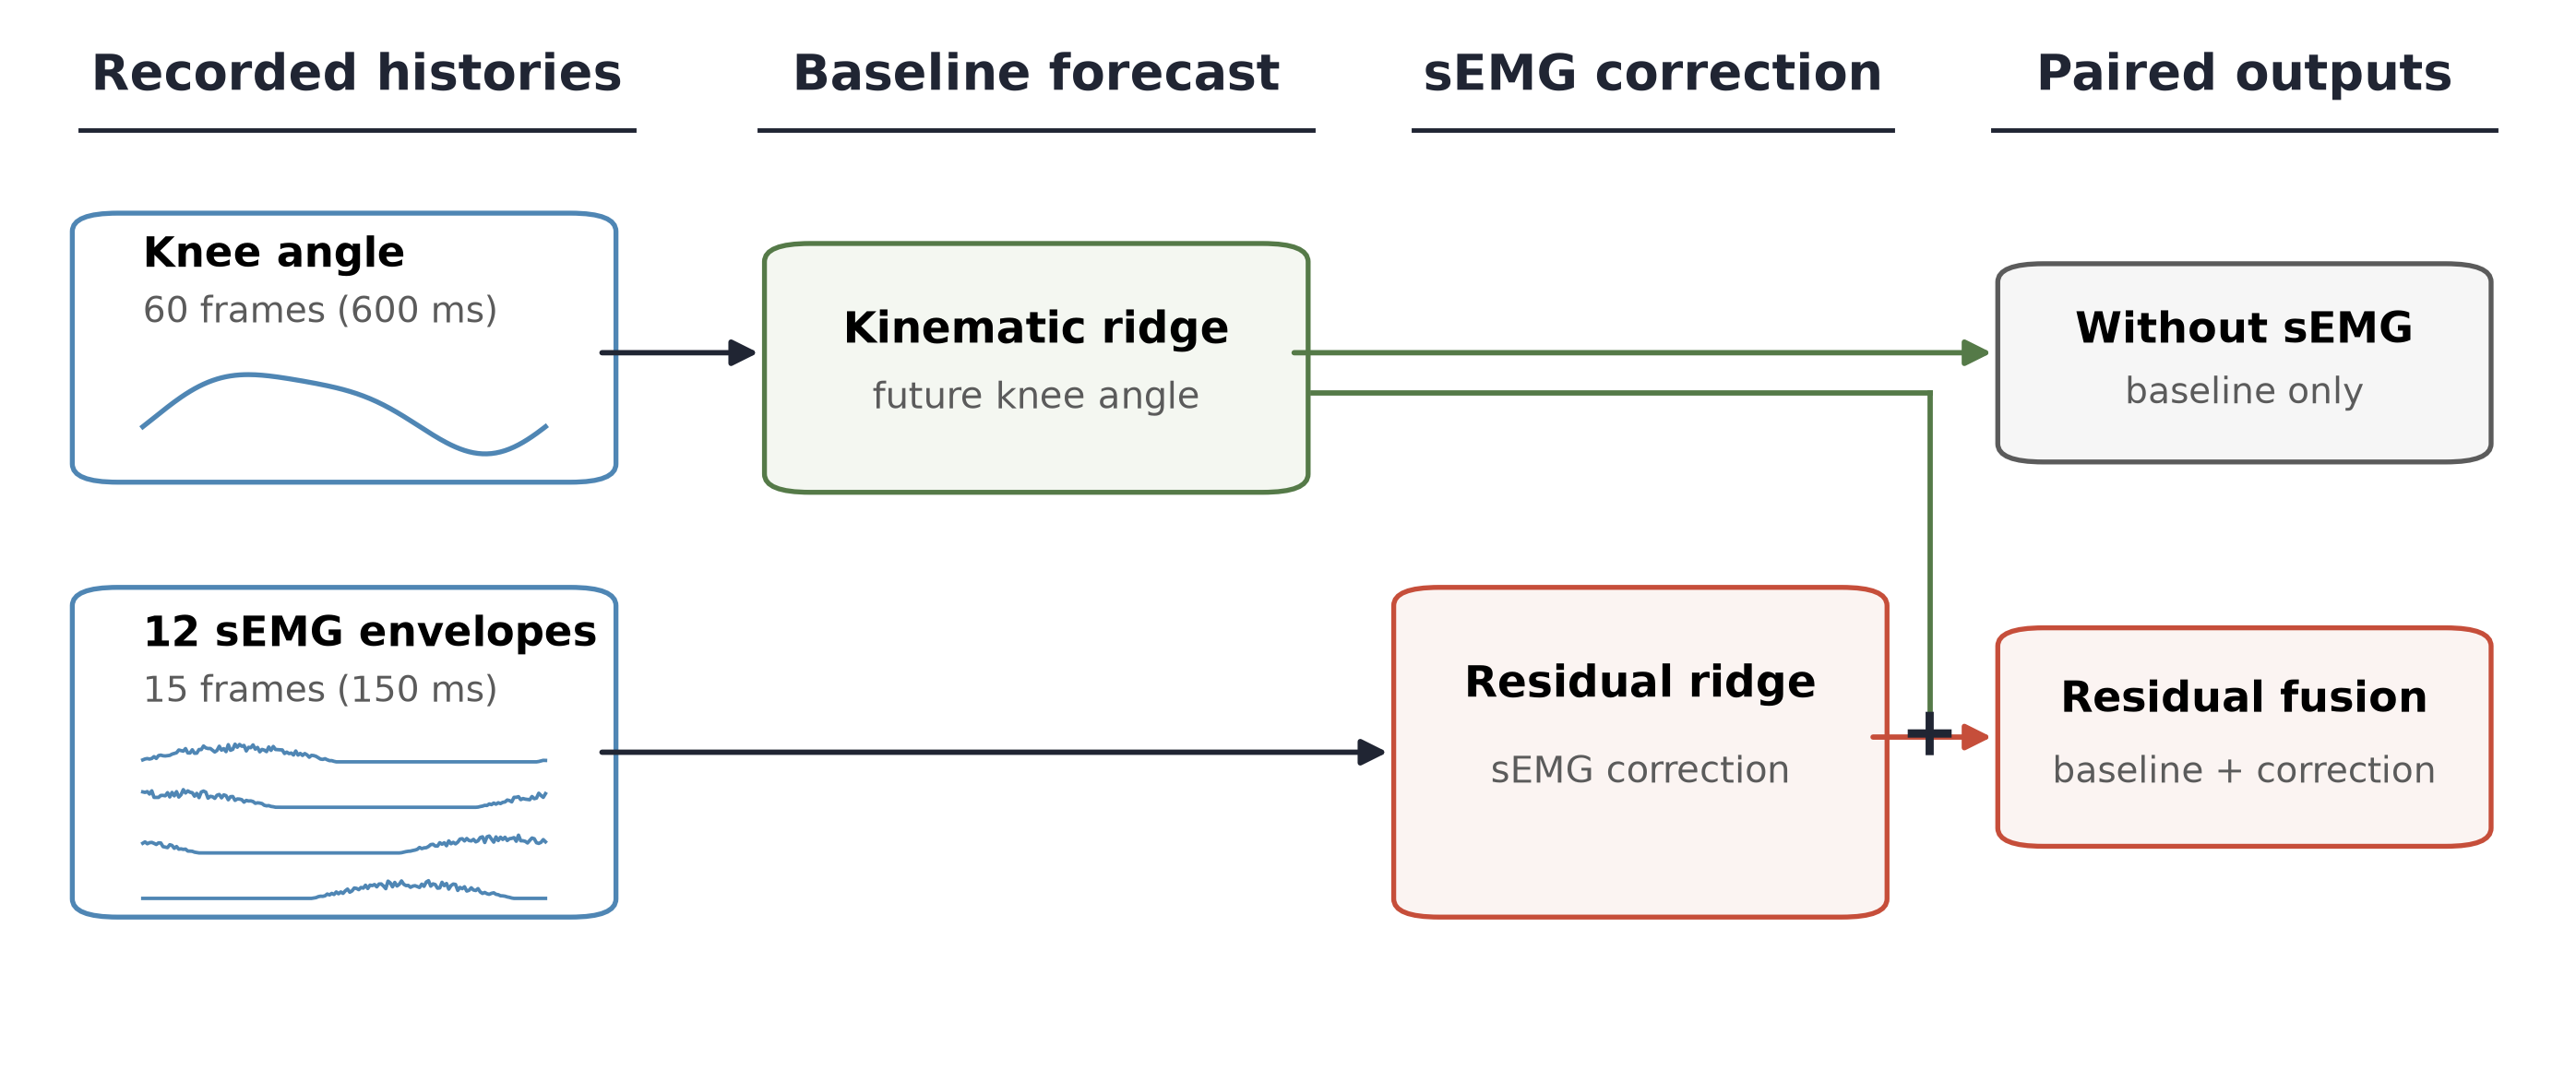
\includegraphics[width=\textwidth]{model_architecture.png}
\caption{\textbf{Residual-fusion model.} Both conditions used the same kinematic prediction; the ablation removed only the sEMG correction.}
\label{fig:model}
\end{figure}

The development search considered ridge penalties from 0.01 to 1,000,000 in powers of ten and residual weights from 0 to 1 in increments of 0.1. Mean participant RMSE on development trial 4 selected a kinematic penalty of 0.1, an sEMG penalty of 10, and $\gamma=1$. These values were then used unchanged in the confirmation group. To prevent a linear residual model from requesting a correction larger than the errors it was trained to correct, its raw output passed through a smooth hyperbolic-tangent bound scaled by each participant's 95th-percentile absolute kinematic training residual. The bound was calculated only from trials 1--3 and was applied under the same rule to every participant and later trial. It limited the model output; it did not modify the recorded sEMG or kinematics.

For each participant, the ablation effect was defined as RMSE without sEMG minus RMSE with residual fusion. A positive value therefore meant that adding sEMG improved prediction. The two RMSE values were paired because they came from the same participant, trial, target samples, and kinematic model. A two-sided paired $t$-test tested the null hypothesis that the mean participant-level improvement was zero. The 95\% confidence interval was the corresponding Student-$t$ interval for the mean paired difference, and standardized effect size was reported as Cohen's $d_z$, the mean difference divided by the standard deviation of those differences. The participant differences showed no material departure from normality (Shapiro--Wilk $W=0.984$, $p=0.358$). Wilcoxon signed-rank and exact sign tests were also calculated as sensitivity analyses; they did not change the conclusion and are included in Additional file 2.

Before the confirmation data were examined, the planned requirements were a positive mean improvement, a confidence interval entirely above zero, a two-sided $p\leq0.05$, and improvement in more than half of participants. This prevented a very small effect from being judged only by its $p$-value.

A secondary timing control tested whether an sEMG advantage depended on the recorded timing of muscle activation. Within each continuous trial, the same 150-ms sEMG history was moved 500 ms earlier relative to the kinematic input and target. There was no wraparound or synthesized sample: an example was discarded if the earlier history did not exist. The aligned model was then rescored on exactly the rows available to the shifted model, and the shifted residual model was refit with the same penalty, residual weight, and training trials. This made the aligned-versus-shifted result a comparison of signal timing rather than a comparison of different target rows.

\subsection{Motion Matching and Physics Evaluation}

Motion matching is a standard approach in real-time character animation and the video-game industry, involving the retrieval of the closest motion snippet from a database using similarity metrics \cite{clavet2016}. Prediction accuracy alone did not answer the research question because a model could produce a moderate RMSE while still generating a knee trajectory that destabilized the body when inserted into a whole-body motion. To provide a realistic body context, each Gait120 query was matched to a physically grounded MoCapAct walking clip based on knee angle and right-thigh orientation \cite{wagener2022}. Knee and thigh matching errors were recorded because an imperfect reference match could affect the physics evaluation separately from the predictor.

The physics panel was created from confirmation trial 5 before motion matching or simulation. A query was a one-second segment containing 100 consecutive recorded 100-Hz knee targets, with the full 600-ms kinematic and 150-ms sEMG histories available for every target. Candidate starts were separated by ten frames, or 100 ms. Sixty-five confirmation participants had at least one complete query, producing 283 candidates. A seeded participant-balanced sample selected 80 windows. Every eligible participant contributed one window before any participant contributed a second. Prediction RMSE, participant ablation improvement, motion-match quality, and simulation outcome were not used to choose a window.

MoCapAct is built from the Carnegie Mellon University Motion Capture Database and provides a trained humanoid control policy, called an expert, for each fixed segment of a motion-capture clip \cite{wagener2022}. MoCapAct calls each fixed segment a snippet. The full library contains many activities, so the present reference bank retained only 157 snippets from the 90 clips whose official activity descriptions were unqualified level walking. Sports, stairs, turns, transitions, and every other activity were excluded before prediction simulations were run.

The Gait120 queries and MoCapAct references had different sampling rates. For the matching search only, the 100-Hz query knee and right-thigh pitch curves were evaluated on the 200-Hz MoCapAct matching grid by linear sampling-rate conversion. This operation was necessary to compare the two time grids and was not applied to the stored Gait120 signals, any model input or target, the reported prediction RMSE, or the prediction errors later supplied to MuJoCo. Each candidate location was aligned with a constant angular offset and either a positive or negative knee convention; no amplitude scaling was allowed. Candidates were ranked by knee-angle RMSE. Right-thigh pitch RMSE was recorded separately as a whole-body match-quality measure.

The 12 closest candidates for each query were considered in that order. The unchanged MoCapAct expert for a candidate had to complete the entire interval twice from the same initial state, reproduce the same knee trajectory in both repetitions, remain upright, and keep the XCoM instability score described below under 0.70. The first candidate satisfying these reference-only requirements became that query's reference. This process did not remove prediction failures: neither prediction condition had been simulated, and every later model balance loss remained in the analysis. Mean knee matching RMSE was required to remain below 10$^{\circ}$ and mean right-thigh pitch RMSE below 15$^{\circ}$.

Before either prediction condition was analyzed, ten selected panel windows received a zero-error target. In this systems check, the knee controller was asked to reproduce the trajectory realized by its own matched MoCapAct expert. At least eight of ten windows had to finish without balance loss, keep instability below 0.70, and track the knee target within 10$^{\circ}$ RMSE. If a controller could not reproduce a stable reference when no prediction error was added, a later model failure could not be attributed to the predictor.

For each selected match, the unmodified MoCapAct expert first produced its realized right-knee trajectory $q_{\mathrm{ref}}(t)$. The recorded prediction error was then inserted into that same whole-body motion:

\begin{equation}
q_c(t)=q_{\mathrm{ref}}(t)+s\left[\hat y_c(t)-y(t)\right],
\label{eq:mapping}
\end{equation}

where $c$ denoted residual fusion or the comparison without sEMG, $\hat y_c(t)-y(t)$ was the prediction error on the recorded Gait120 target, and $s\in\{-1,1\}$ converted the Gait120 knee convention to the sign used by the matched MoCapAct knee. This mapping preserved the magnitude and direction of every sampled prediction error while keeping both models inside the same motion produced by a stable MoCapAct expert. It is an offline test of a recorded error, not a proposed real-time prosthetic controller, because a deployed controller would not know the future recorded knee angle $y(t)$.

The 100-Hz Gait120 prediction timeline and 33.33-Hz MuJoCo control timeline had an exact three-frame relationship. Frames 0, 3, 6, and so forth were therefore selected directly. No prediction supplied to the simulator was interpolated, clipped, scaled, or refit. A moving-target proportional-derivative controller applied

\begin{equation}
\tau=K_p(q_{\mathrm{des}}-q)+K_d(\dot q_{\mathrm{des}}-\dot q),
\end{equation}

with $K_p=800$, $K_d=40$, and a force limit of 800. The proportional term corrected knee-angle error, while the derivative term corrected error relative to the changing target velocity. Desired velocity was the backward difference between the current and preceding targets and was set to zero at the first control step to avoid an artificial handoff impulse. The gains and force limit came from the original implementation and were checked on development walking clips before the confirmation panel. They were not adjusted using confirmation prediction or instability outcomes.

The residual-fusion and without-sEMG simulations for a given Gait120 window used the same MoCapAct snippet and start time, expert policy, initial body state, simulator state, warm-up, and knee controller. Only the Gait120 knee-error trajectory in Eq.~\ref{eq:mapping} changed. The unmodified MoCapAct expert supplied a third reference simulation for calculating added instability. The numerical evaluation contained all 80 windows at each of seven prediction-accuracy checkpoints, producing 560 checkpoint-window simulations. Complete recordings were additionally rendered for eight evenly spaced panel indices chosen before results were known: 0, 11, 22, 33, 44, 55, 66, and 77.

\begin{figure}[!htbp]
\centering
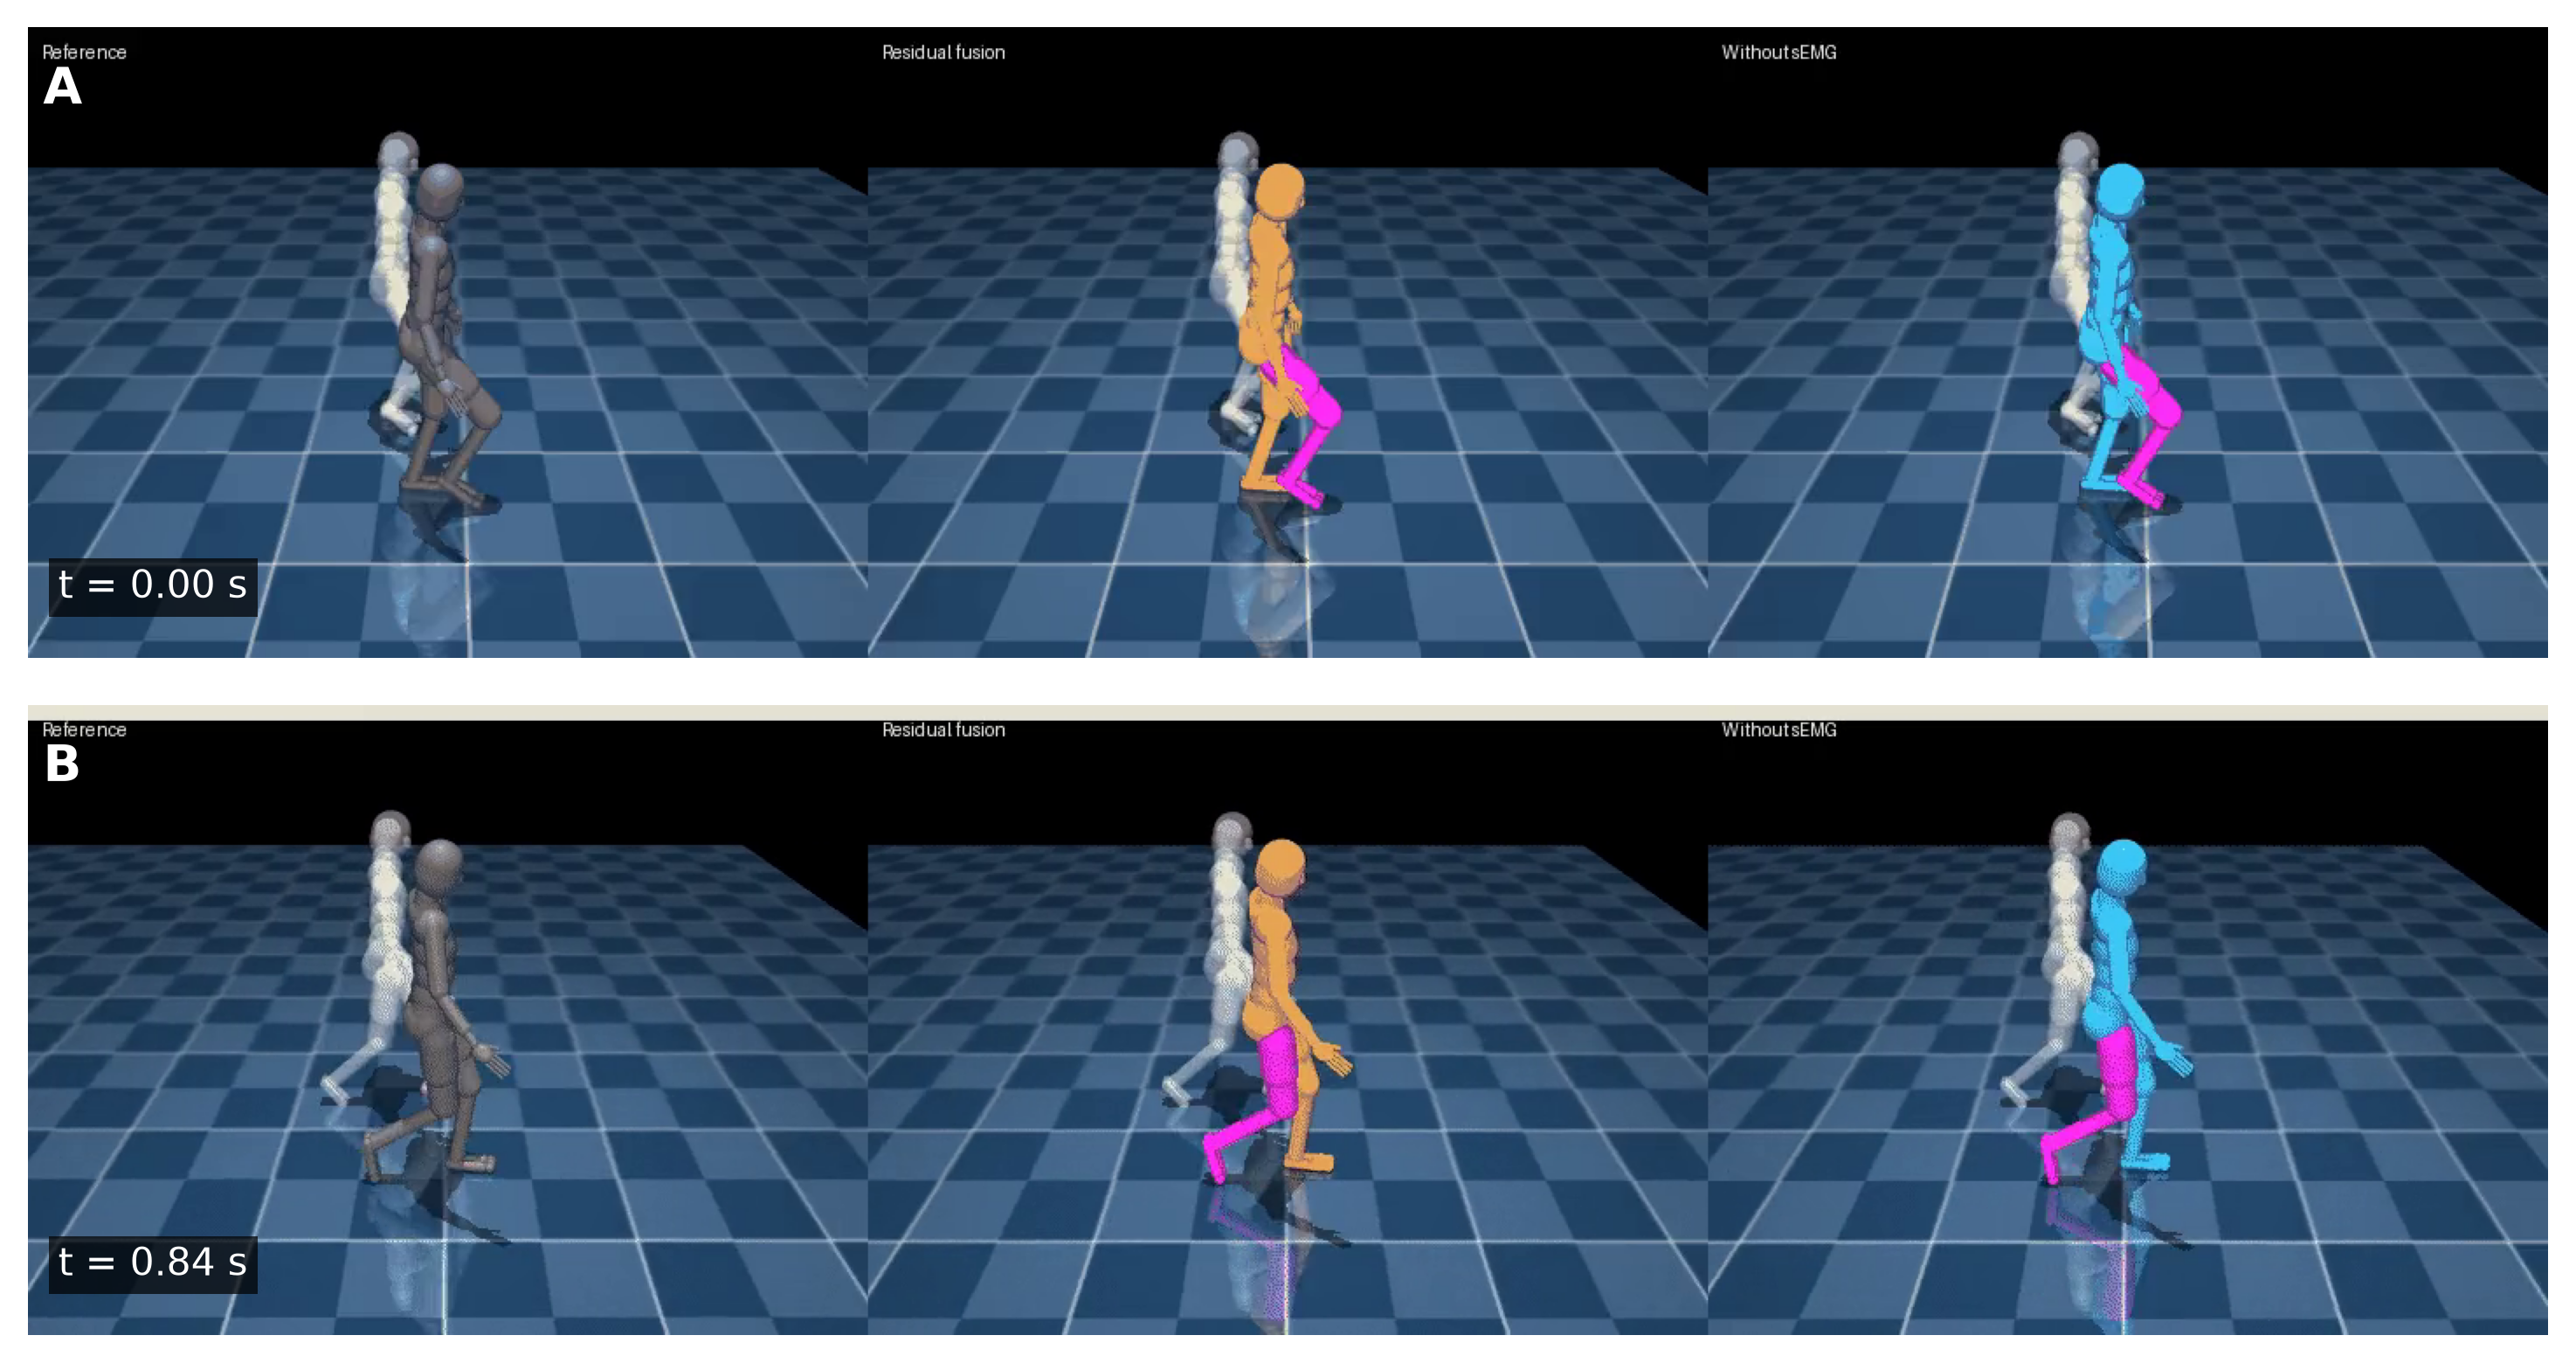
\includegraphics[width=0.98\textwidth]{simulation_sequence.png}
\caption{\textbf{Recorded simulation sequence.} The matched reference, residual-fusion condition, and without-sEMG condition at the beginning and end of one final S083 trial-5 simulation. The magenta right leg received the knee target.}
\label{fig:simseq}
\end{figure}

\begin{figure}[!htbp]
\centering
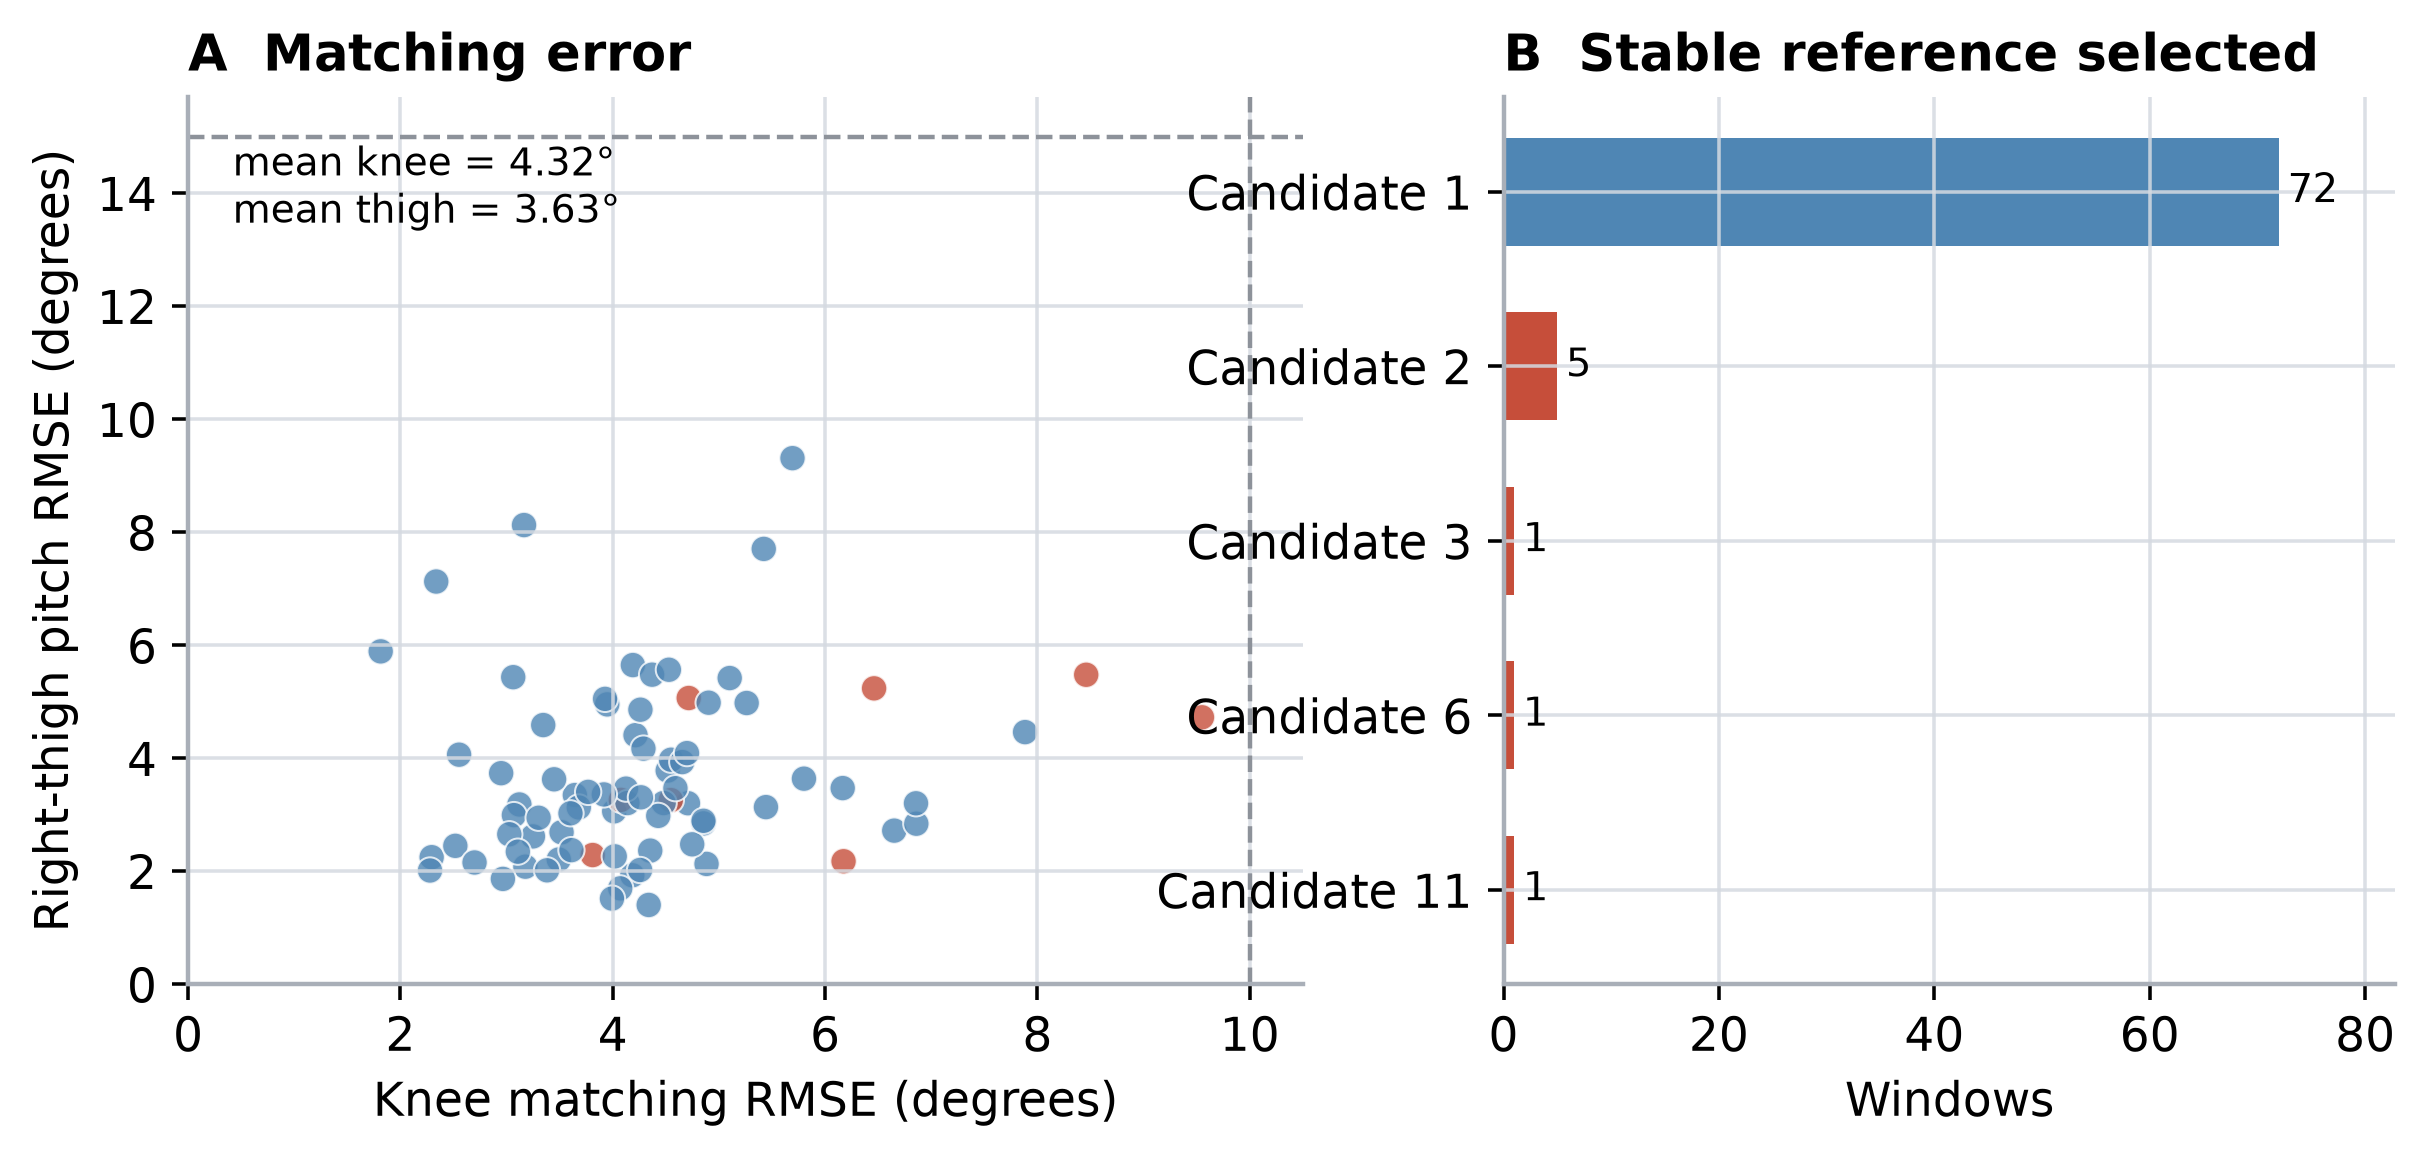
\includegraphics[width=0.98\textwidth]{motion_matching_quality.png}
\caption{\textbf{Motion matching.} Knee and right-thigh pitch errors for the 80 Gait120-to-MoCapAct matches.}
\label{fig:matching}
\end{figure}

\subsection{Evaluating Simulations with an Instability Metric}

At each control step, the convex hull of the current foot--ground contact points defined the support polygon. The extrapolated center of mass extends the horizontal CoM position in the direction of its velocity:

\begin{equation}
\mathrm{XCoM}=\mathrm{CoM}+\frac{v_{\mathrm{CoM}}}{\sqrt{g/l}},
\end{equation}

where $v_{\mathrm{CoM}}$ is horizontal center-of-mass velocity, $g$ is gravitational acceleration, and $l$ is the instantaneous pendulum length from the support plane to the center of mass \cite{hof2005,hof2008}. The signed XCoM support margin was the shortest horizontal distance from the XCoM to the boundary of the support polygon. It was positive when the XCoM was inside the polygon and negative when it was outside \cite{curtze2024}.

\begin{figure}[!htbp]
\centering
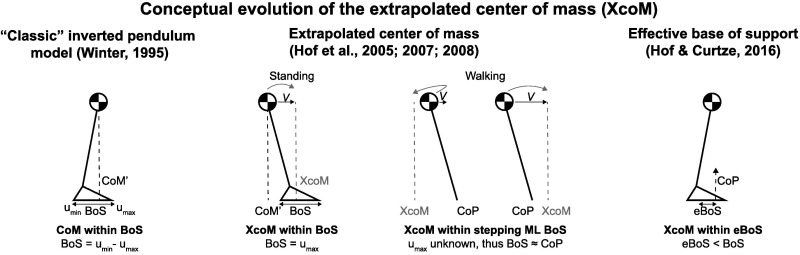
\includegraphics[width=0.94\textwidth]{xcom_concept.png}
\caption{\textbf{Extrapolated center of mass.} XCoM includes CoM velocity relative to the support polygon \cite{hof2005,hof2008}.}
\label{fig:xcom}
\end{figure}

The per-step instability score was constrained to $[0,1]$ and combined three features from the preceding ten control steps: the smallest support margin in that interval, the ending margin, and the rate at which the margin was moving outward. Their fixed weights were 0.55, 0.25, and 0.20. These definitions, thresholds, and weights were inherited from the original implementation and were not adjusted using Gait120 prediction outcomes. The score is a simulation measure, not a clinical probability of falling. A balance loss was recorded when the smoothed score remained at least 0.85 for four consecutive control steps. This persistence requirement distinguished a sustained loss of support from a single brief boundary crossing.

\begin{figure}[!htbp]
\centering
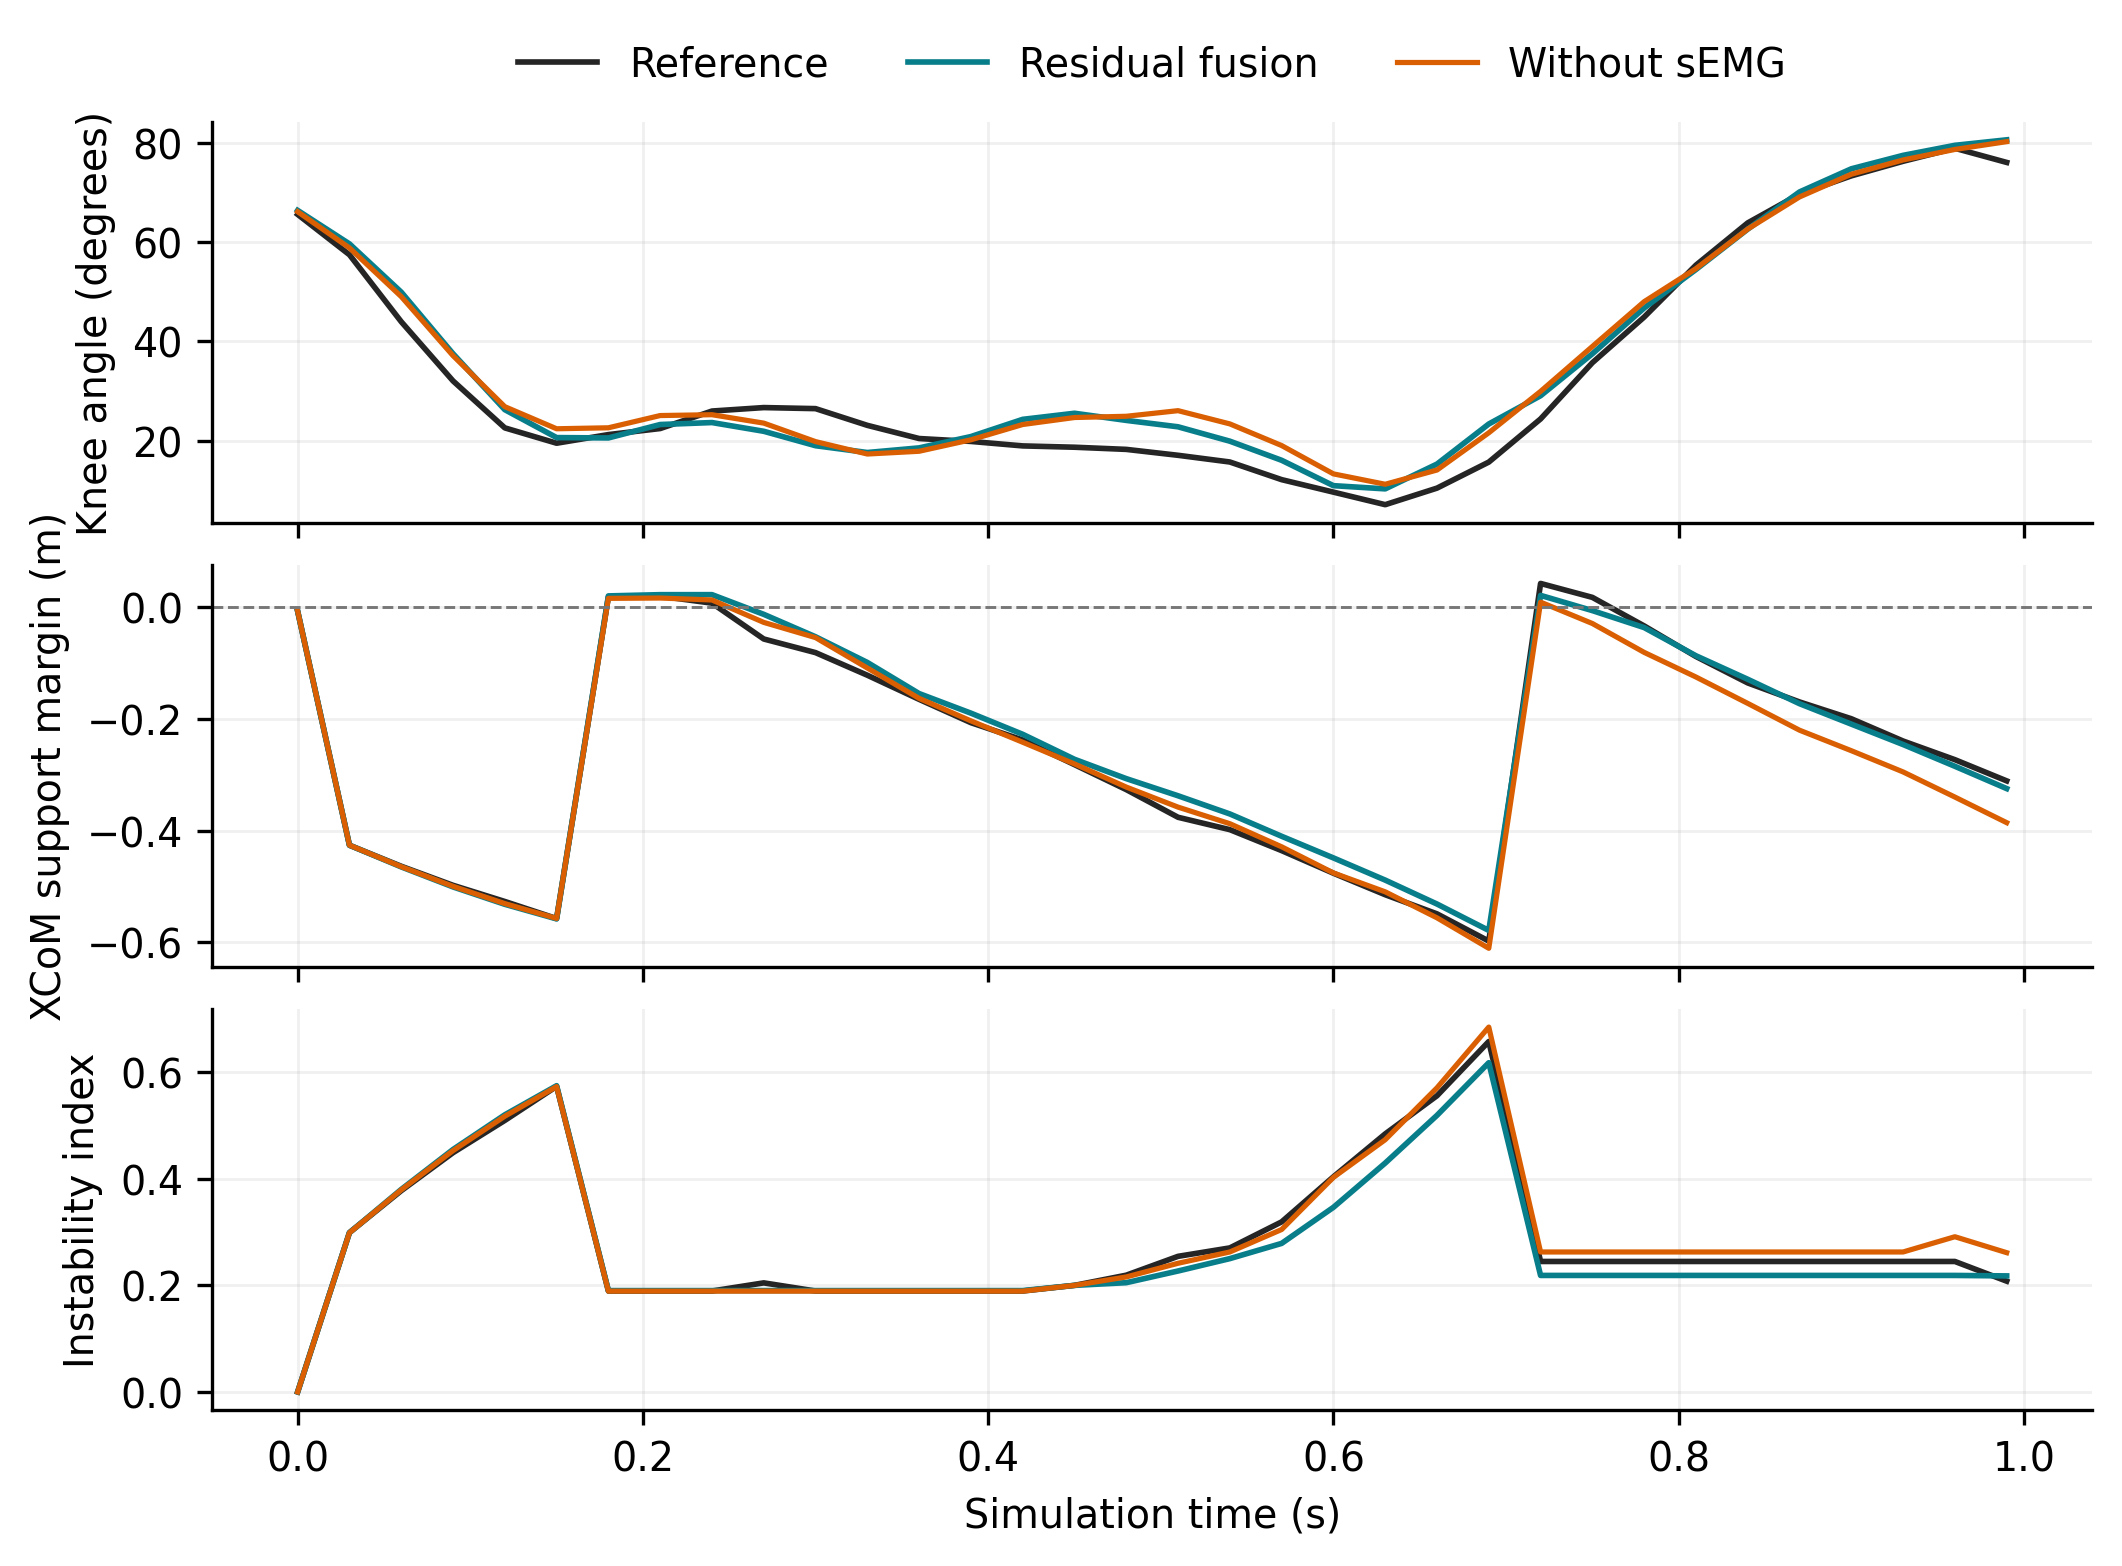
\includegraphics[width=0.98\textwidth]{simulation_metrics.png}
\caption{\textbf{Simulation measurements.} Knee angle, XCoM support margin, and instability from the recorded S083 sequence.}
\label{fig:simmetrics}
\end{figure}

The instability area under the curve (AUC) was calculated by trapezoidal integration of the score over simulation time. It therefore measured both the size and duration of instability, in score-seconds. A matched MoCapAct reference can have nonzero instability without any prediction error, so the primary outcome subtracted that window's own reference AUC:

\begin{equation}
AUC_{\mathrm{excess},c}=AUC_c-AUC_{\mathrm{reference}}.
\end{equation}

This value was called excess-instability AUC. A value above zero meant that a prediction condition was more unstable than its matched MoCapAct reference, while a value below zero meant it was less unstable. Every model balance loss and early termination remained in the analysis.

\subsection{Correlation Study}

The primary physical comparison used the full-data model. Residual-fusion excess AUC was compared with without-sEMG excess AUC for the same window. When a participant contributed two windows, the values were averaged first so that each of the 65 participants contributed one value to statistical inference. The paired physical effect was defined as without-sEMG excess AUC minus residual-fusion excess AUC; a positive value favored residual fusion. A two-sided paired $t$-test tested whether the mean participant-level difference was zero, and the corresponding Student-$t$ interval provided its 95\% confidence interval.

The next analysis asked whether a participant with lower prediction RMSE also produced less excess instability. Spearman correlation was used because it tests whether two quantities change monotonically without requiring a linear relationship \cite{spearman1904}. Motion matching introduces a separate error: a poor Gait120-to-MoCapAct match could raise instability even if the predictor were accurate. The analysis therefore accounted for knee matching RMSE and right-thigh pitch RMSE with the Frisch--Waugh--Lovell (FWL) procedure in rank space \cite{frisch1933,lovell1963}. First, prediction RMSE, excess-instability AUC, knee matching RMSE, and thigh matching RMSE were replaced by their participant ranks. Ranked prediction RMSE and ranked excess AUC were then separately regressed on both ranked matching errors. Finally, the residuals from those two regressions were correlated. The resulting partial Spearman coefficient describes the remaining RMSE--instability relationship after the measured knee and thigh matching relationships have been removed. Its confidence interval used 20,000 participant-bootstrap resamples, and its two-sided $p$-value used 100,000 participant permutations.

The full-data model occupied a narrow RMSE range, which could hide a relationship that appears only after prediction becomes much worse. To widen the range without changing the model, target participants, or simulation panel, the same model was refit using the first 5\%, 10\%, 20\%, 40\%, 60\%, 80\%, and 100\% of each participant's eligible training examples in recorded order. These fractions were chosen before the physics results were available. All seven versions predicted the same trial-5 windows and entered the same MoCapAct matches.

Because only seven accuracy checkpoints were simulated, the accuracy-path analysis reports the adjacent measured RMSE values that bracketed a simultaneous marked increase in mean excess AUC and balance losses. Values inside an unsampled interval were not treated as measured results. The result is therefore an observed transition interval rather than an exact clinical cutoff.

The analysis was performed with Python 3.12, NumPy 2.5, SciPy, and MuJoCo 2.2.2. An AI-assisted coding tool was used for software development, code review, and language editing. The author checked the data flow, statistical outputs, figures, citations, and final manuscript and accepts responsibility for the work.

\FloatBarrier

\section{Results}\label{sec:results}

\subsection{Prediction Accuracy}

In the 90-participant confirmation group, mean RMSE was 4.748$^{\circ}$ with residual fusion and 5.093$^{\circ}$ without sEMG. Adding sEMG therefore reduced participant RMSE by an average of 0.345$^{\circ}$ (95\% confidence interval 0.252--0.438$^{\circ}$; paired $t(89)=7.39$, $p=7.50\times10^{-11}$; Cohen's $d_z=0.78$). Seventy of 90 participants improved (Fig.~\ref{fig:ablation}). The sensitivity analyses reached the same conclusion (Wilcoxon signed-rank $p=1.53\times10^{-9}$; exact sign $p=1.14\times10^{-7}$). The positive mean effect, confidence interval above zero, significant paired test, and improvement in more than half of participants satisfied the planned ablation requirements.

\begin{figure}[!htbp]
\centering
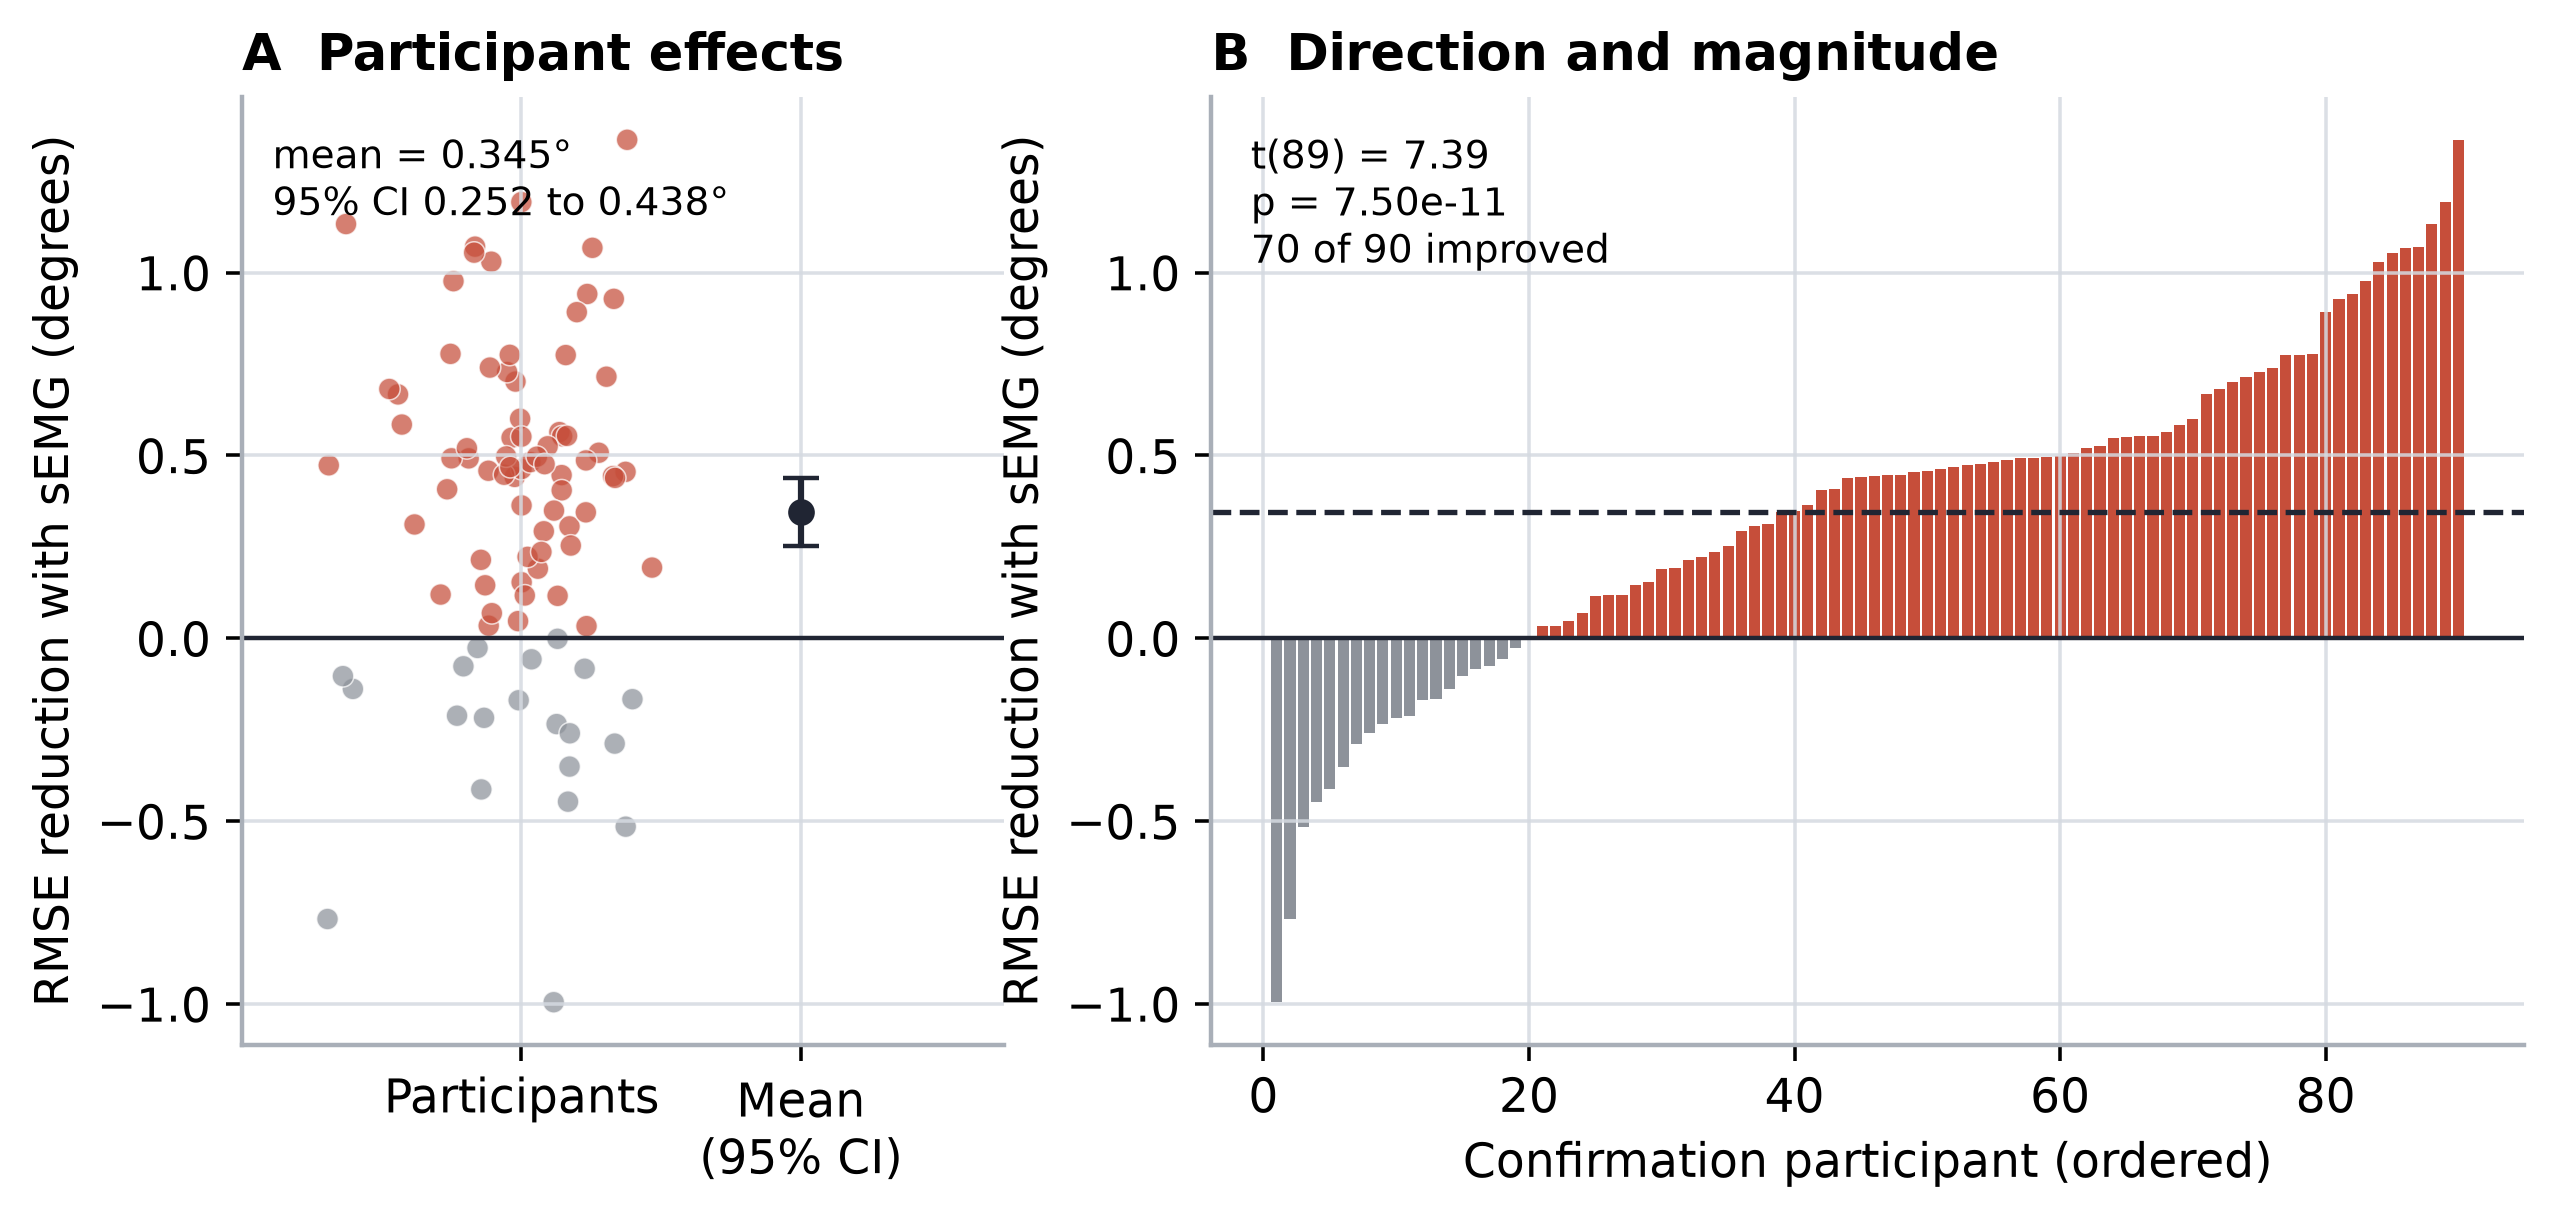
\includegraphics[width=0.96\textwidth]{prediction_ablation.png}
\caption{\textbf{sEMG ablation.} Participant-level RMSE reduction after adding sEMG. Positive values favor residual fusion; the point and error bar in panel A show the mean and 95\% confidence interval.}
\label{fig:ablation}
\end{figure}

The 500-ms timing control did not support a specifically timed pre-activation interpretation. Sixty-six participants had trial-5 recordings long enough to contain both the original sEMG history and the history shifted 500 ms earlier. On these identical target rows, aligned sEMG improved RMSE by 0.209$^{\circ}$ (95\% confidence interval 0.079--0.331$^{\circ}$; 45 of 66 participants improved). The earlier sEMG history improved RMSE by 0.294$^{\circ}$ (95\% confidence interval 0.190--0.395$^{\circ}$; 50 of 66 participants improved). The direct difference, shifted-sEMG RMSE minus aligned-sEMG RMSE, was $-0.085^{\circ}$ (95\% confidence interval $-0.202$ to 0.030$^{\circ}$; paired $t(65)=-1.42$, $p=0.160$). The primary ablation therefore shows that sEMG added predictive information beyond knee history, but the timing control does not show that this advantage came specifically from the recorded timing of pre-activation.

\subsection{Motion Matching and Paired Simulation}

All 80 Gait120 windows received a level-walking reference from the MoCapAct expert-policy library. Mean knee matching RMSE was 4.317$^{\circ}$ and mean right-thigh pitch RMSE was 3.630$^{\circ}$, below the planned 10$^{\circ}$ and 15$^{\circ}$ limits (Fig.~\ref{fig:matching}). The matches used 29 MoCapAct snippets. The first-ranked candidate was stable for 72 windows. In the other eight windows, the first candidate failed the reference-only replay and the next stable candidate in the knee-RMSE ranking was used. When prediction error was set to zero, the knee controller reproduced all ten selected reference motions without balance loss.

The experiment contained 560 simulations: 80 fixed windows at each of seven training-data checkpoints. At the full-data checkpoint, neither the unmodified references nor the zero-error controller checks lost balance. Two residual-fusion simulations and two without-sEMG simulations met the balance-loss definition. Figure~\ref{fig:simexamples} shows three of the eight windows recorded for visual documentation.

\begin{figure}[!htbp]
\centering
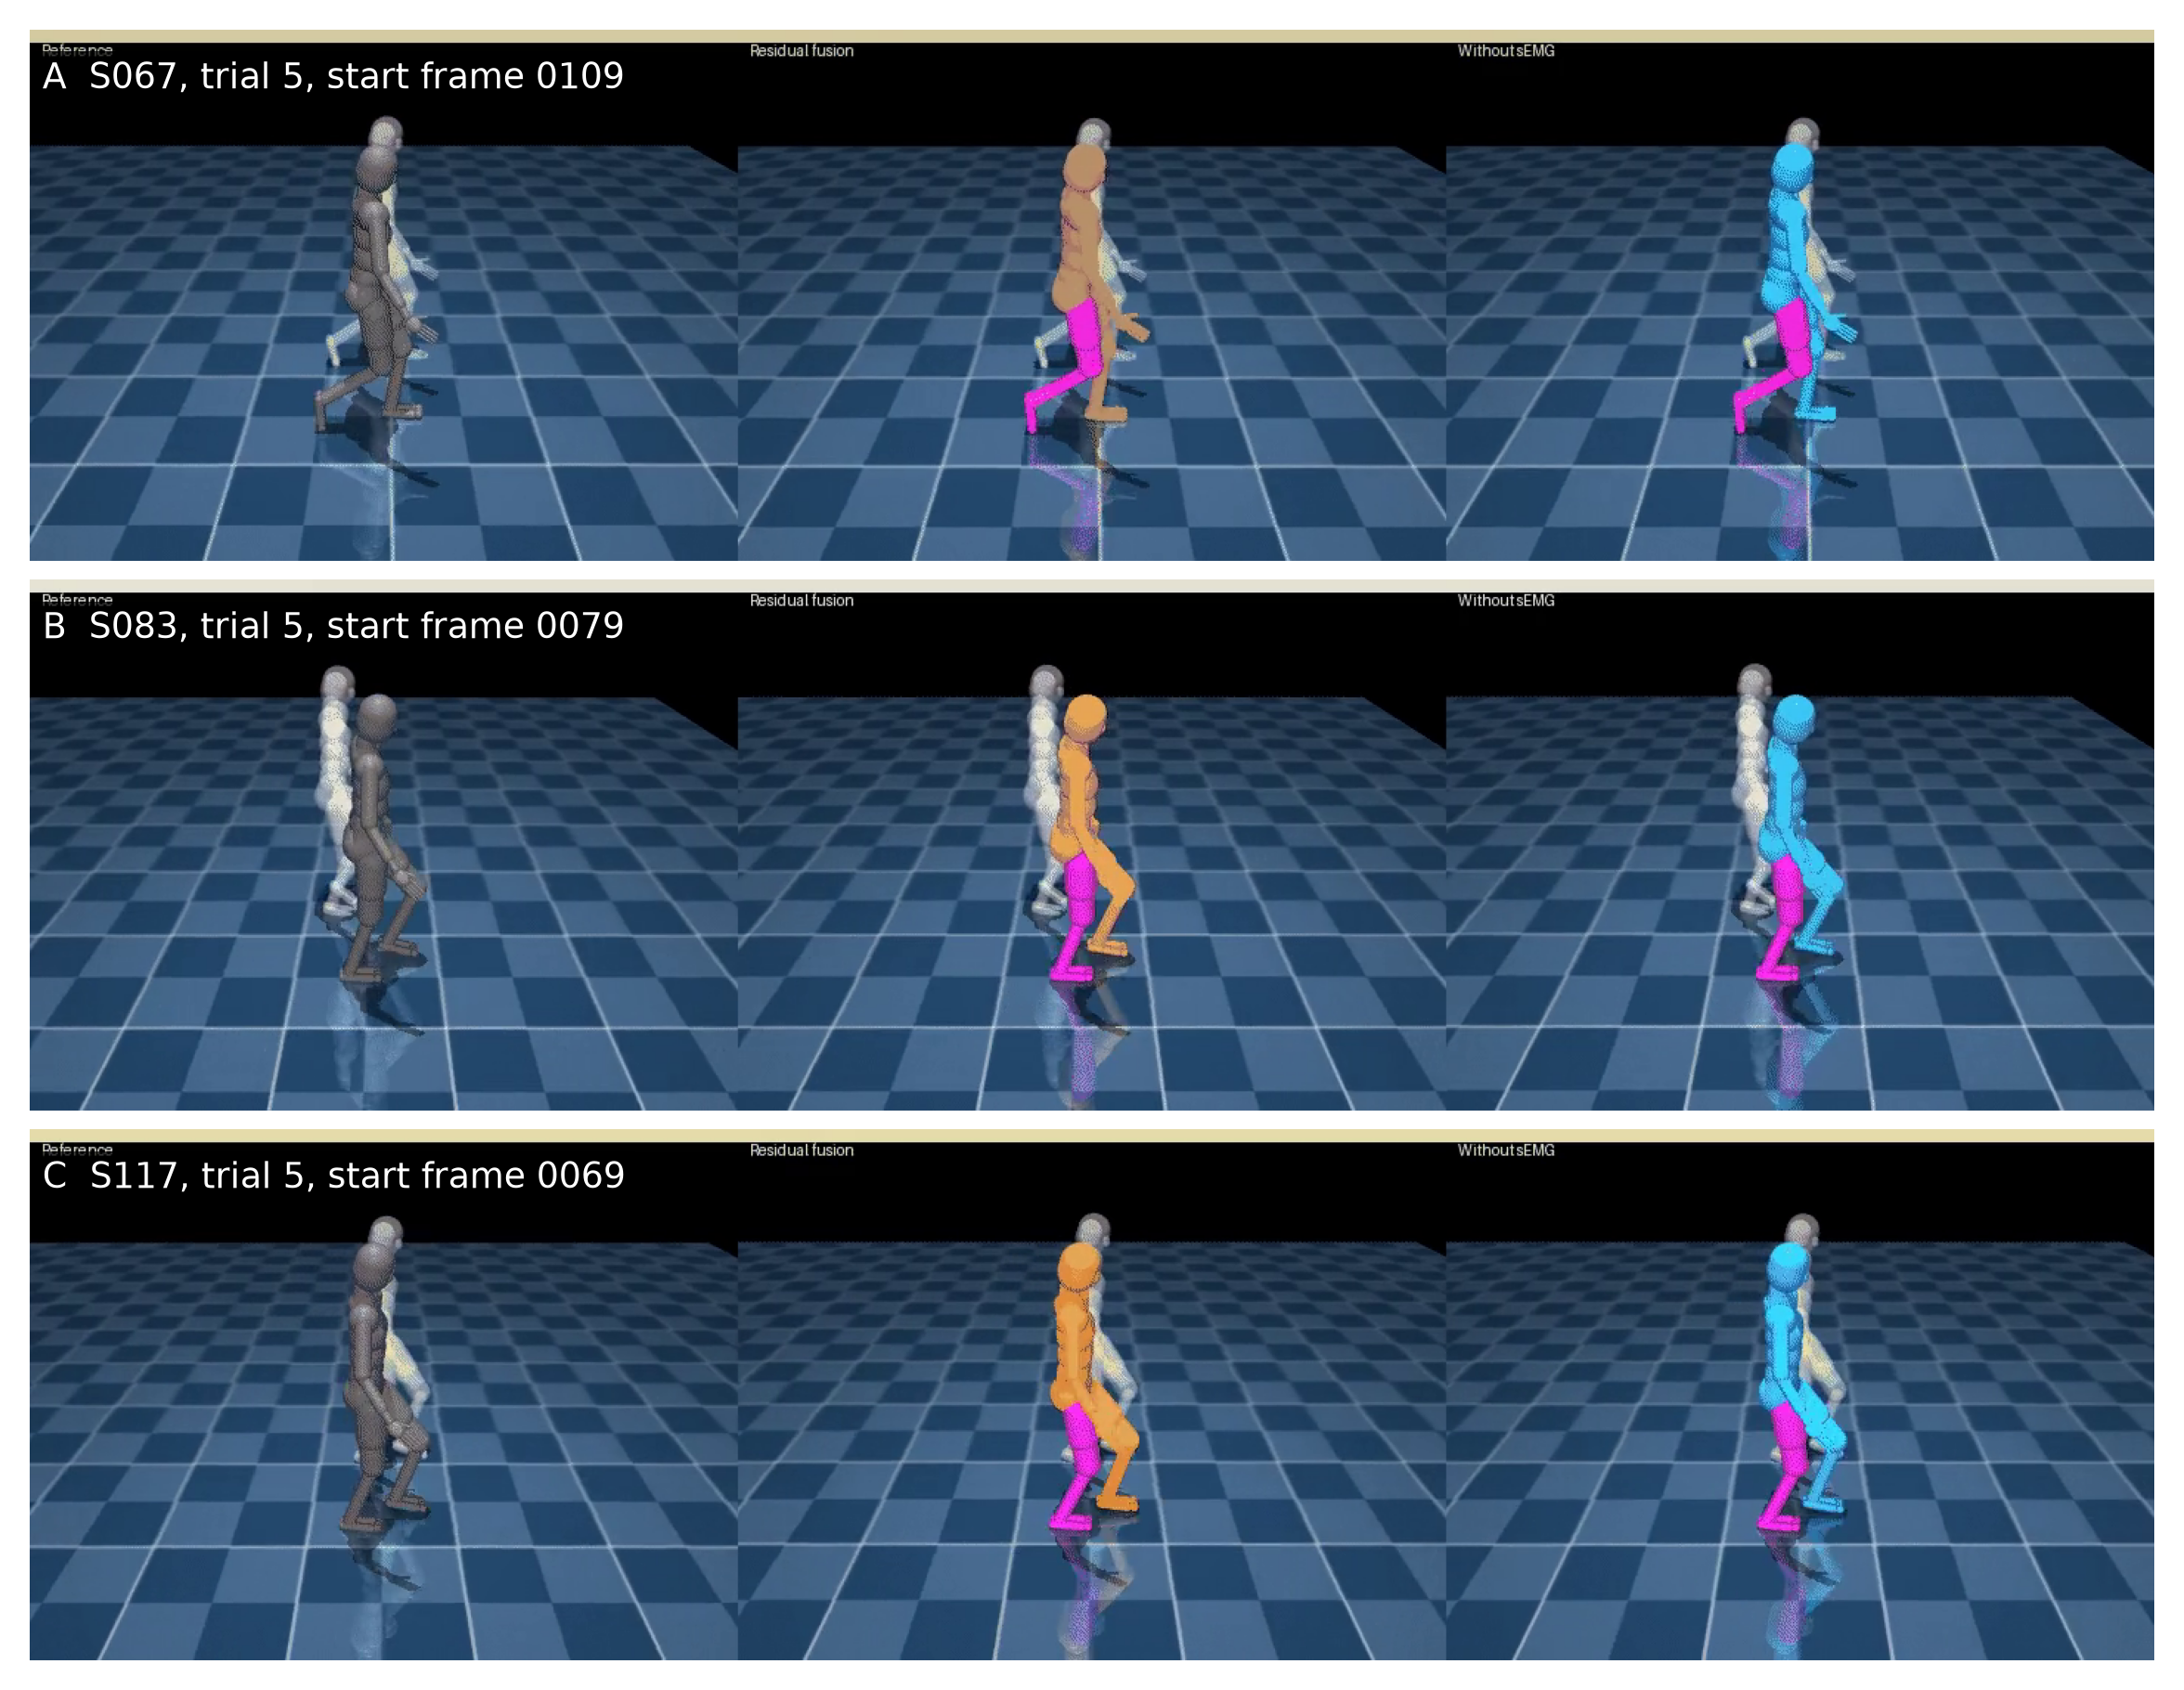
\includegraphics[width=0.98\textwidth]{simulation_representatives.png}
\caption{\textbf{Recorded simulation examples.} Three final MoCapAct reference, residual-fusion, and without-sEMG comparisons.}
\label{fig:simexamples}
\end{figure}

Mean residual-fusion excess-instability AUC was 0.0215 score-seconds (95\% confidence interval 0.0066--0.0375). The corresponding value without sEMG was 0.0204 score-seconds (95\% confidence interval 0.0058--0.0350). The mean paired reduction, defined as without-sEMG excess AUC minus residual-fusion excess AUC, was $-0.0012$ score-seconds (95\% confidence interval $-0.0105$ to 0.0081; paired $t(64)=-0.25$, $p=0.801$). Thirty-five of 65 participants had lower excess AUC with fusion (Fig.~\ref{fig:physics}). The confidence interval included zero and the observed mean was close to zero. Therefore, the confirmed 0.345$^{\circ}$ prediction improvement did not produce a detectable reduction in simulated instability.

\begin{figure}[!htbp]
\centering
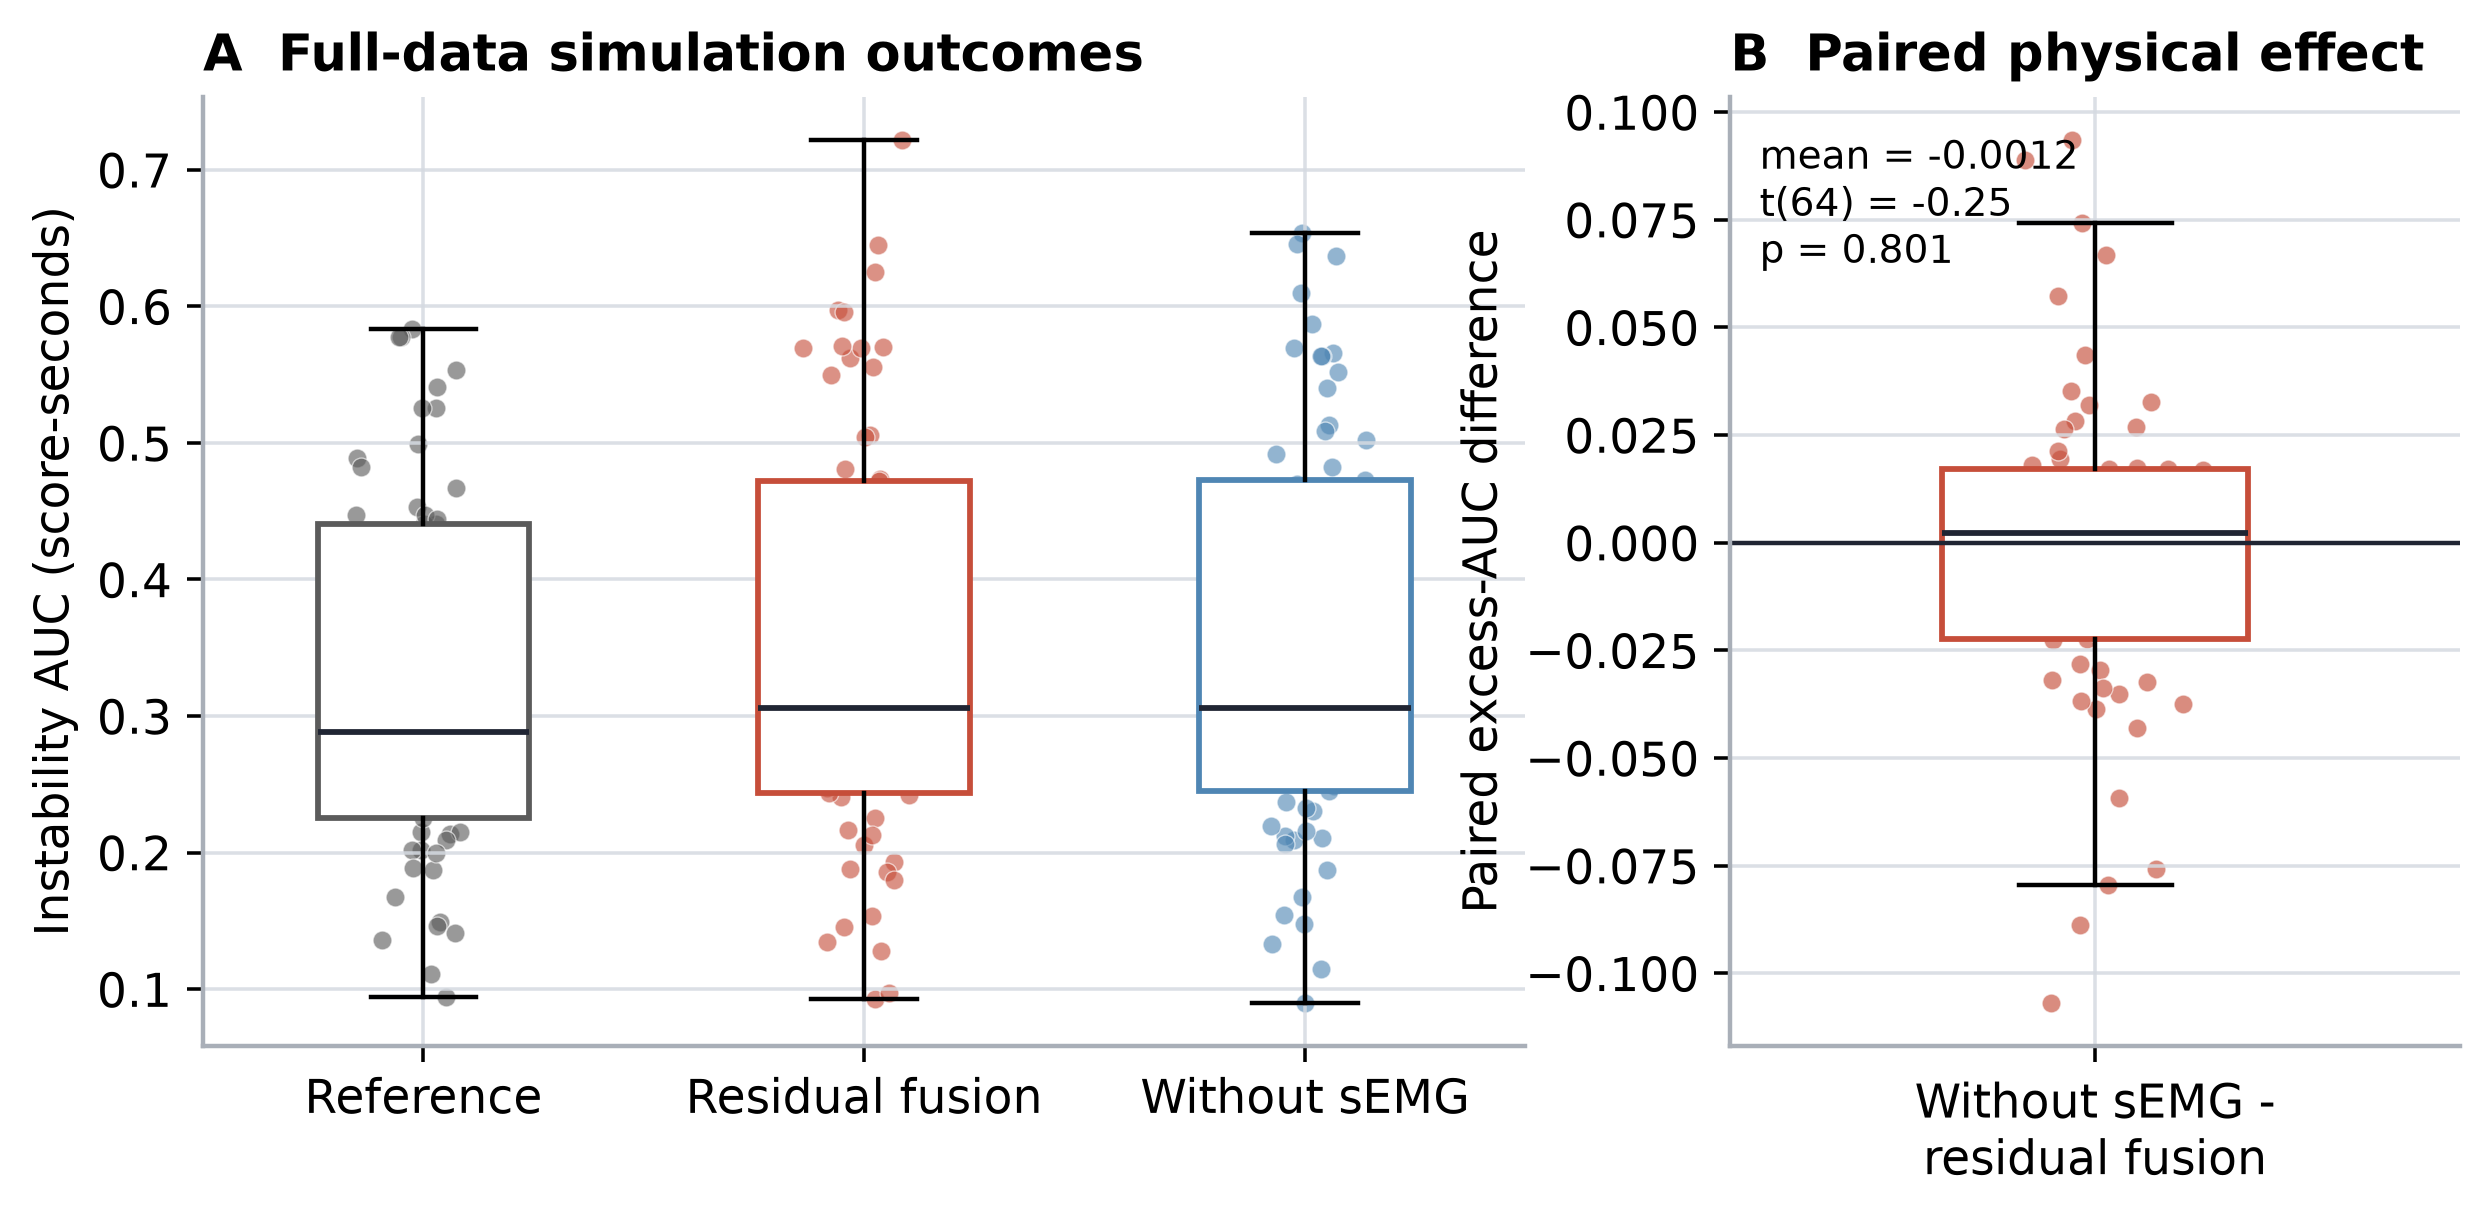
\includegraphics[width=0.98\textwidth]{simulation_outcomes.png}
\caption{\textbf{Paired simulation outcomes.} Participant-level excess-instability AUC and the difference between prediction conditions.}
\label{fig:physics}
\end{figure}

\subsection{Prediction Error vs. Excess Instability}

The raw participant-level association between residual-fusion RMSE and excess instability was weak (Spearman $\rho=-0.117$, $p=0.355$; Fig.~\ref{fig:correlations}A). After knee matching RMSE and right-thigh pitch RMSE were accounted for, partial Spearman $\rho$ was $-0.145$ (95\% confidence interval $-0.370$ to 0.082; permutation $p=0.248$; Fig.~\ref{fig:correlations}C). The confidence interval included zero, and the point estimate was slightly negative rather than positive. Within the full-data model's RMSE range, a participant with lower prediction error did not reliably produce less excess instability.

\begin{figure}[!htbp]
\centering
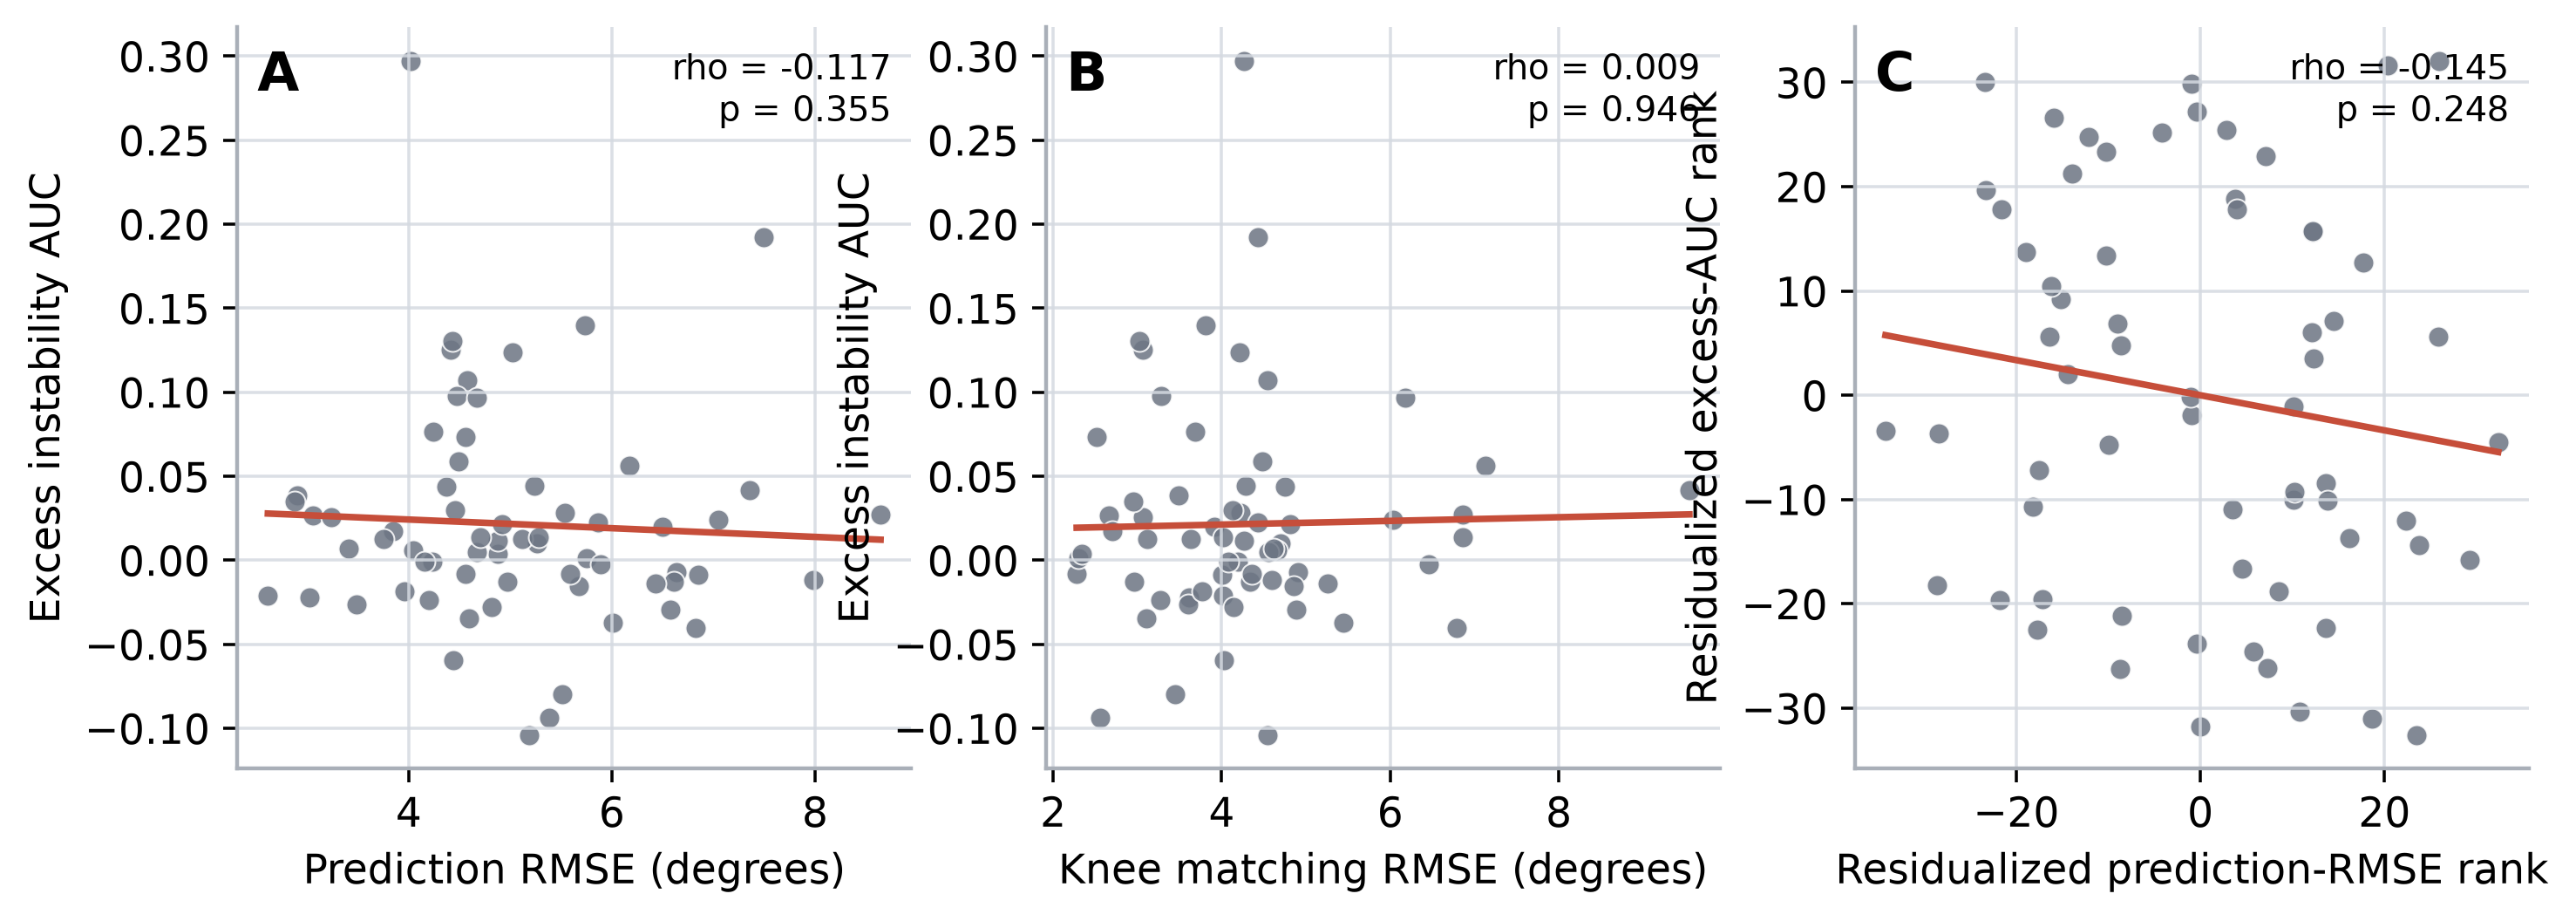
\includegraphics[width=0.99\textwidth]{correlation_analysis.png}
\caption{\textbf{Prediction error and instability.} Panel C shows the relationship after knee and thigh matching errors were removed in rank space.}
\label{fig:correlations}
\end{figure}

\subsection{Prediction Accuracy Across the Training Range}

Prediction RMSE decreased as more participant training data were used (Fig.~\ref{fig:training}). The 5\% and 10\% models produced 16.29$^{\circ}$ and 13.41$^{\circ}$ RMSE, respectively. From 20\% onward, mean RMSE remained near 5$^{\circ}$. These seven versions created the wider accuracy range needed to determine whether the weak full-data correlation was limited to an already accurate model.

\begin{figure}[!htbp]
\centering
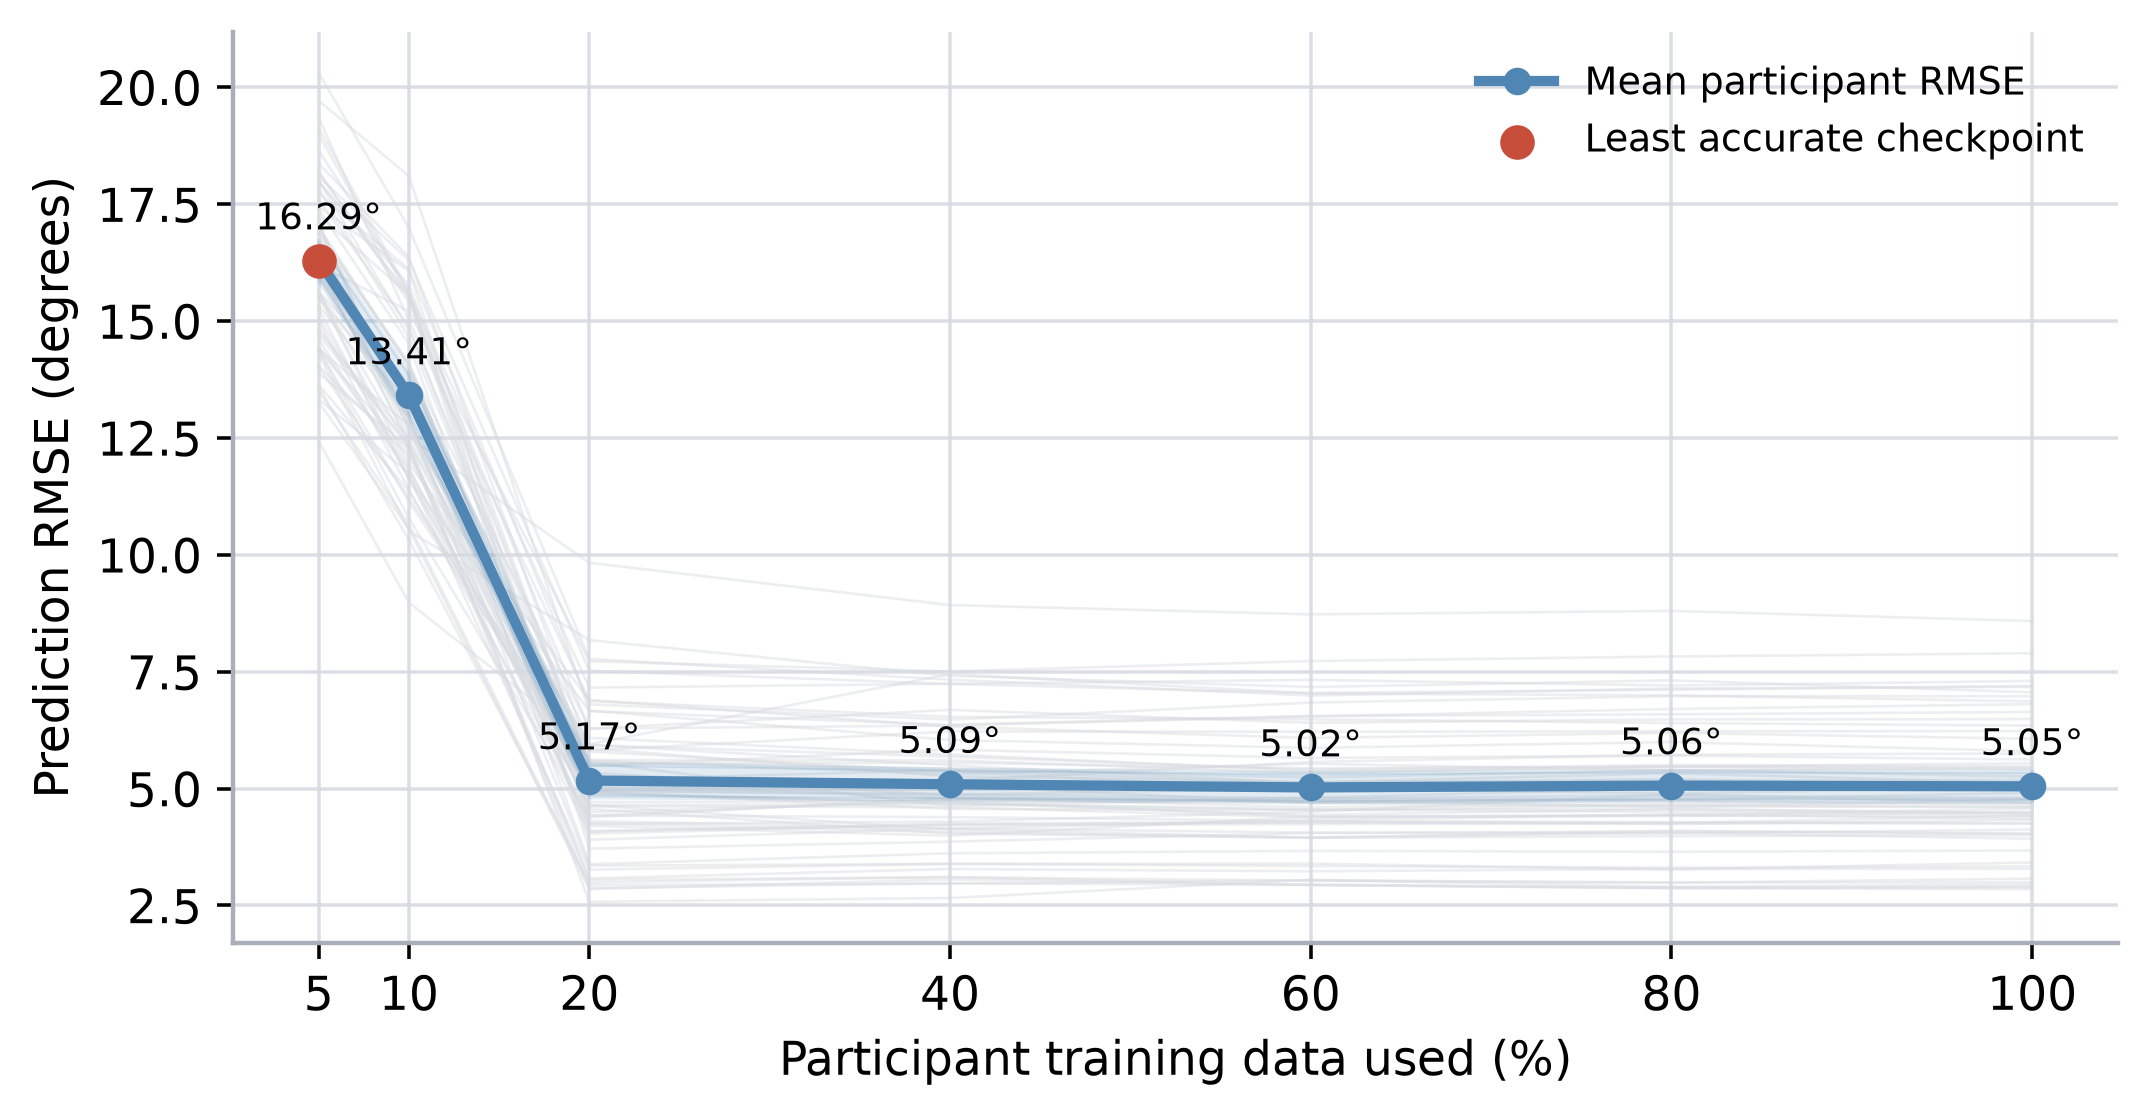
\includegraphics[width=0.98\textwidth]{training_rmse.png}
\caption{\textbf{RMSE across training-data fractions.} Gray lines show individual participants and the blue line shows the participant mean at each checkpoint.}
\label{fig:training}
\end{figure}

The physical result changed sharply at the least accurate checkpoint (Table~\ref{tab:path}; Fig.~\ref{fig:path}). At 16.29$^{\circ}$ RMSE, mean excess AUC was 0.137 and 32 of 80 windows lost balance. At 13.41$^{\circ}$ RMSE, mean excess AUC was 0.015 and three windows lost balance. The 20\% through 100\% checkpoints produced mean excess AUC values between 0.015 and 0.022 and one or two balance losses. The direct observations therefore place the marked physical deterioration between 13.41$^{\circ}$ and 16.29$^{\circ}$ RMSE. No checkpoint was run inside that 2.89$^{\circ}$ interval, so the experiment does not identify a more exact boundary.

\begin{table}[!htbp]
\caption{\textbf{Prediction accuracy and physical outcome by training-data checkpoint}}\label{tab:path}
\begin{tabular}{@{}rrrr@{}}
\toprule
Training data (\%) & RMSE ($^{\circ}$) & Excess AUC & Balance losses \\
\midrule
5   & 16.29 & 0.137 & 32 \\
10  & 13.41 & 0.015 & 3 \\
20  & 5.17  & 0.015 & 1 \\
40  & 5.09  & 0.019 & 1 \\
60  & 5.02  & 0.021 & 2 \\
80  & 5.06  & 0.021 & 2 \\
100 & 5.05  & 0.022 & 2 \\
\botrule
\end{tabular}
\end{table}

The two adjacent checkpoints that showed the change therefore bracket an observed transition between 13.41$^{\circ}$ and 16.29$^{\circ}$ RMSE (Fig.~\ref{fig:path}). This range is the clearest limit supported by the experiment. It should not be reduced to one exact value because no checkpoint was simulated inside the interval.

\begin{figure}[!htbp]
\centering
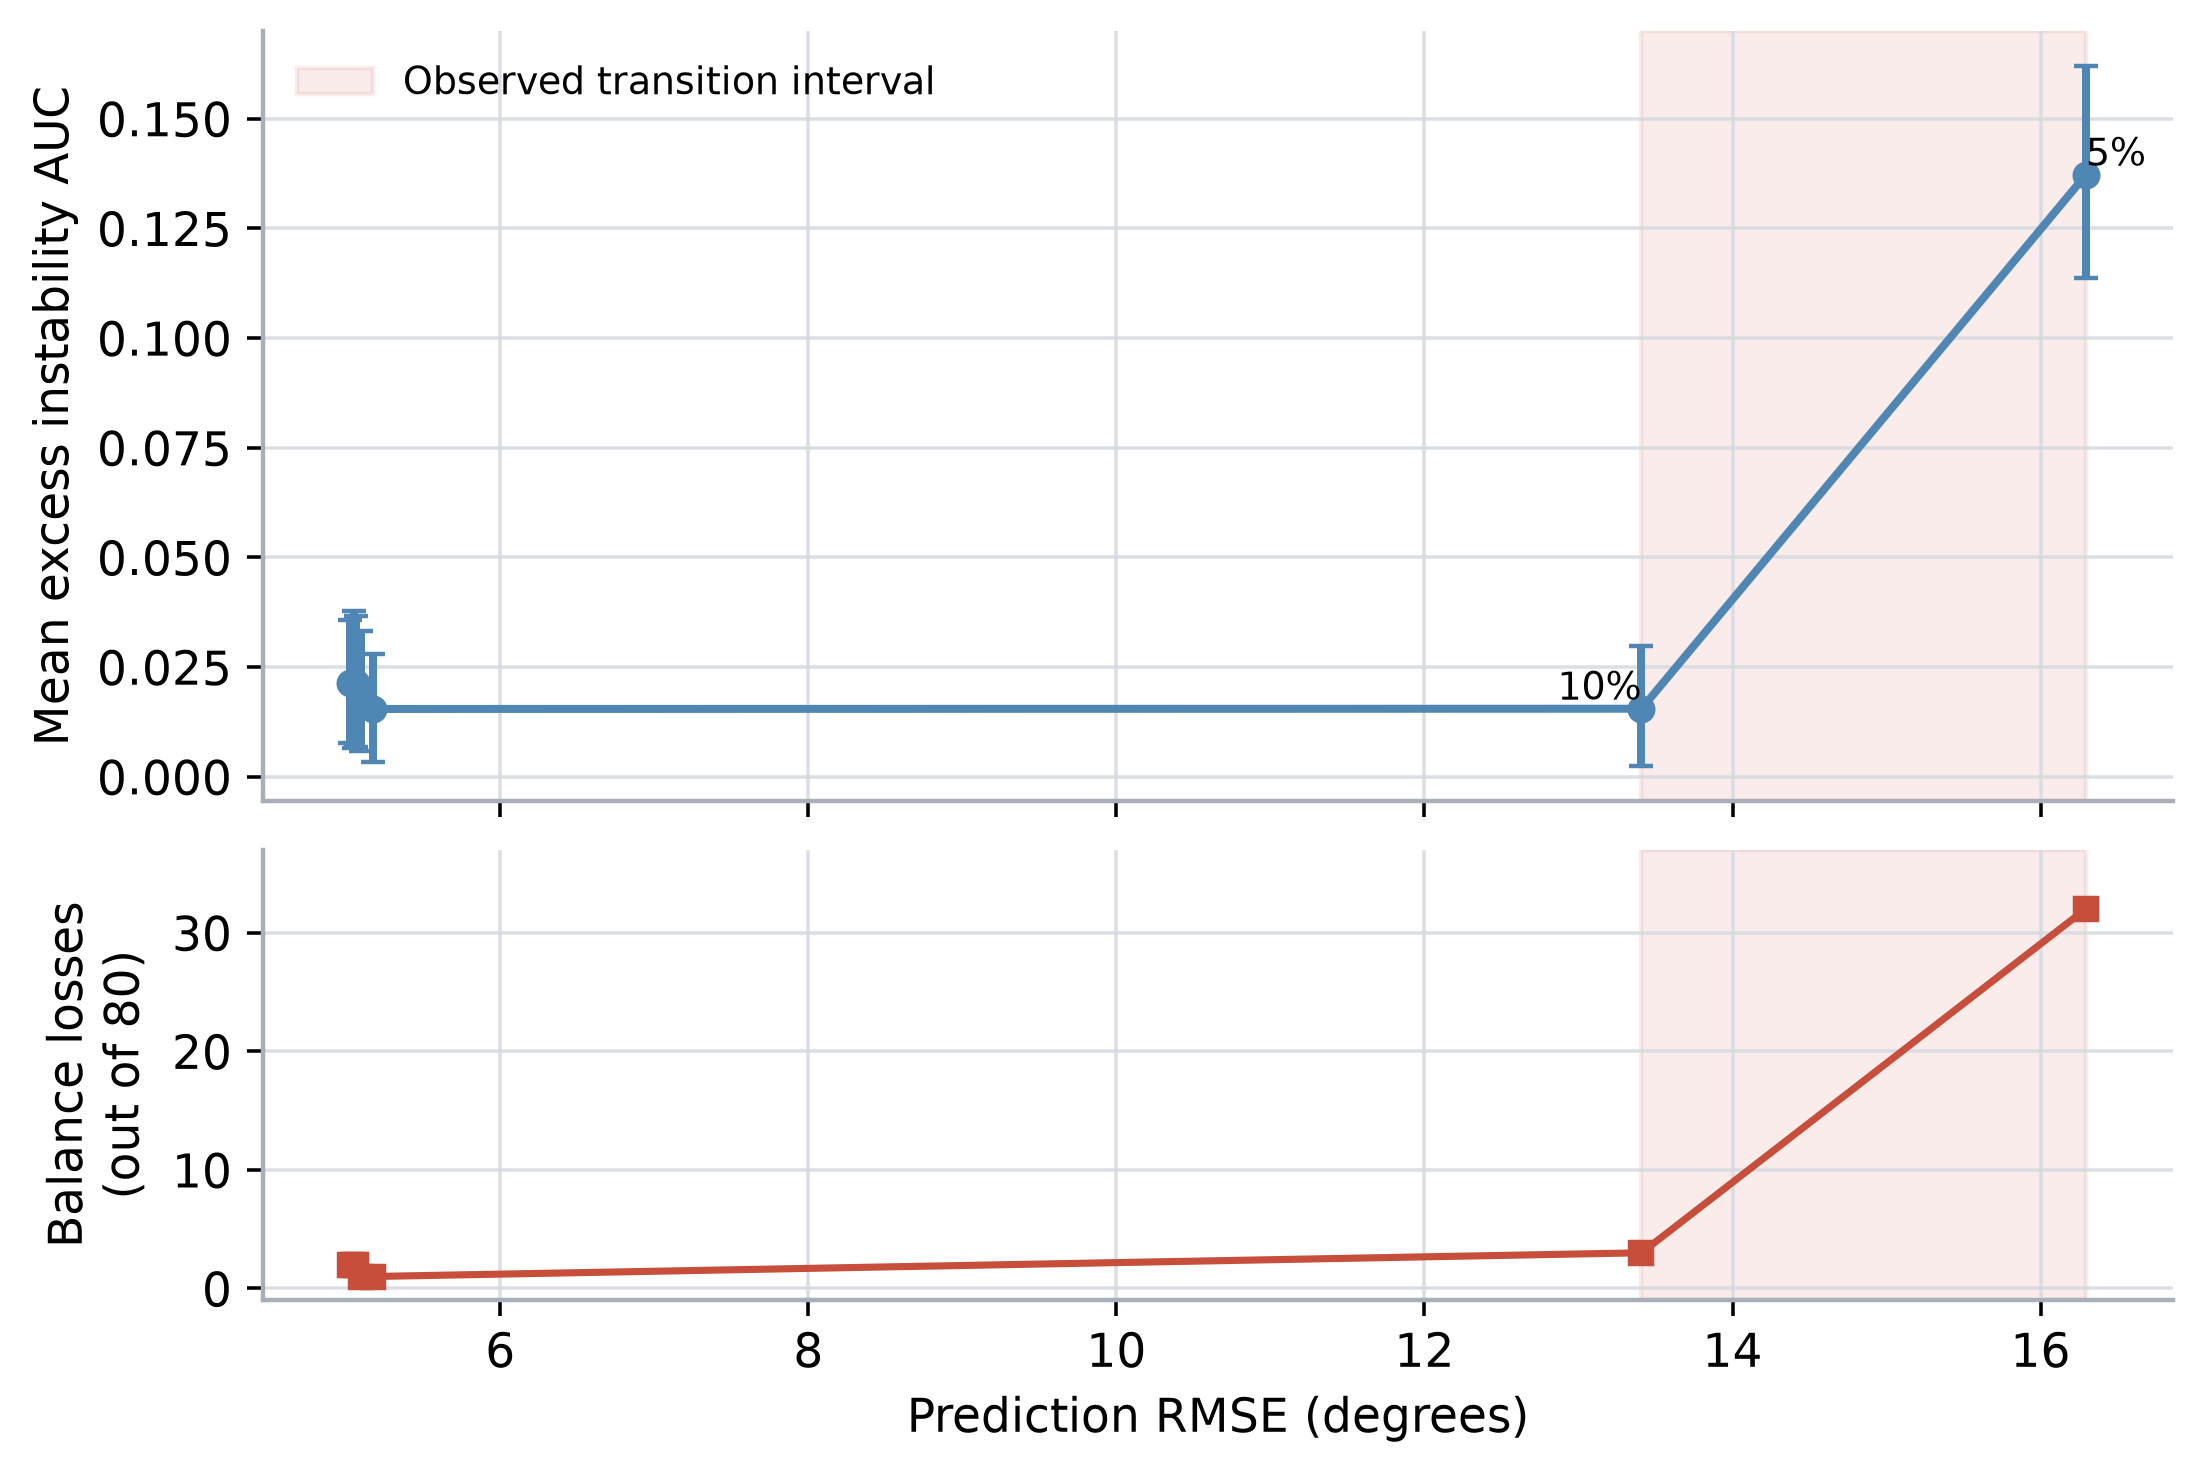
\includegraphics[width=0.98\textwidth]{accuracy_transition.png}
\caption{\textbf{Physical behavior across RMSE.} The shaded region marks the interval between the adjacent checkpoints where excess instability and balance losses increased sharply.}
\label{fig:path}
\end{figure}

\FloatBarrier

\section{Discussion}\label{sec:discussion}

This study tested whether a statistically reliable improvement in sEMG-based knee-angle prediction also corresponded to lower excess instability in a physics-based prosthetic simulation. The prediction ablation succeeded. At 100 ms ahead, residual fusion reduced participant RMSE by 0.345$^{\circ}$ on average, its confidence interval remained above zero, and 70 of 90 confirmation participants improved. This result is consistent with the central finding of multimodal knee-prediction studies by Sun et al. and Yi et al., which reported that myoelectric information can add value beyond kinematics alone \cite{sun2022,yi2022}. It also corrects the main weakness of the earlier version of this project, in which removing sEMG did not make prediction worse.

The physical result was different. The residual-fusion model and the same model without sEMG were tested in the same MoCapAct walking motion, from the same initial simulator state, with only the right-knee prediction error changed. Under that comparison, the mean excess-instability difference was $-0.0012$ score-seconds and its confidence interval included zero. The 0.345$^{\circ}$ prediction gain was therefore real as an offline reduction in error, but too small to produce a measurable stability gain in this simulation. This finding follows the distinction raised in virtual myoelectric-control studies: offline accuracy can establish that a model predicts well without establishing that a modest improvement will change whole-body function \cite{hargrove2007,krasoulis2019}.

Several explanations are plausible. Whole-body locomotion is constrained by more than the right knee angle, so a small local improvement may not matter if the trunk, contralateral leg, support configuration, and MoCapAct policy state already define a stable motion. RMSE also does not retain the direction or gait phase of each error. Two trajectories can have similar RMSE while placing their largest errors during different parts of swing, stance, or support transition, and those parts of the gait cycle do not contribute equally to balance. Finally, the full-data model occupied a narrow range near 5$^{\circ}$ RMSE, leaving little variation from which to estimate a relationship with a whole-body outcome.

The timing control narrows what can be claimed about the sEMG result. Moving the sEMG history 500 ms earlier did not remove its predictive advantage. The ablation therefore shows that the sEMG channels contained repeatable information not present in knee history alone, but it does not show that the improvement came specifically from correctly timed pre-activation. Stable differences in activation between participants or trials may have helped the residual model even after temporal alignment was disrupted.

The wider accuracy experiment clarifies why a positive ablation and a null physical comparison can occur together. Models between approximately 5$^{\circ}$ and 13$^{\circ}$ RMSE produced similar mean excess instability and few balance losses. The 16.29$^{\circ}$ checkpoint was different: mean excess AUC increased to 0.137 and 32 of 80 windows lost balance. The simulations therefore showed a direct physical deterioration between measured checkpoints at 13.41$^{\circ}$ and 16.29$^{\circ}$ RMSE. The present result does not show that RMSE is irrelevant; it shows that small RMSE differences among already accurate models need not correspond to detectable differences in this simulation.

This does not mean that simulation should replace predictive benchmarking. A predictor still needs to be accurate and its sEMG contribution still needs to generalize to held-out data. Simulation adds a separate test of what the remaining error does when it is inserted into a controlled whole-body motion. The appropriate evaluation sequence is therefore predictive accuracy, motion-match quality, and then paired physical behavior.

\subsection{Limitations}

Several limitations constrain how far the present conclusions should be generalized. First, the Gait120 participants were healthy adult males, not transfemoral prosthesis users. The study therefore evaluated a prosthetic-testing method with able-bodied walking data, and generalization to amputee physiology or socket-mounted sensing requires new data. Second, the model was participant calibrated with trials 1--3 and does not test immediate transfer to a wearer who provided no calibration. Third, only level walking was studied. This restriction was necessary to keep the Gait120 queries and MoCapAct references within the same activity, but it narrows the conclusion to ordinary walking.

The residual-fusion model was designed for this study rather than copied from one published architecture. Its simplicity made the sEMG ablation direct, but the 0.345$^{\circ}$ improvement should not be assumed for another model or dataset. In addition, the timing control prevents a causal claim that the improvement came specifically from correctly timed pre-activation.

The motion matcher used sampling-rate conversion and constant coordinate alignment to compare Gait120 with the MoCapAct library. These operations were limited to the reference search, but they mean that a match is an aligned similarity rather than an identical recording. The 80 windows used 29 MoCapAct snippets, so some windows shared a reference policy. The one-second simulations measured the immediate response to prediction error rather than long-term recovery or repeated gait cycles.

Finally, the instability score is an XCoM-based simulation measure, not a clinical probability of falling. Although its definitions and thresholds came from the original implementation and every prediction balance loss was retained, another whole-body outcome could emphasize different errors. The seven accuracy checkpoints also leave unresolved intervals. The study should therefore be read as evidence that the RMSE--stability relationship changes across the measured accuracy range, not as a clinical RMSE safety threshold.

\subsection{Future Work}

The clearest direction for future work is to narrow the interval where prediction error began to matter physically. Additional checkpoints between 13.41$^{\circ}$ and 16.29$^{\circ}$ would locate the directly observed deterioration more precisely.

Another extension would be to move from able-bodied level-walking data to recordings from transfemoral prosthesis users while preserving the same paired reference and prediction evaluation structure. Future studies should also examine phase-sensitive error measures, such as stance-weighted RMSE or event-aligned error around support transitions. The present result does not prove that every prediction metric is equally limited. It shows that participant-level RMSE within the final model's narrow range did not independently explain excess instability.

\section{Conclusion}\label{sec:conclusion}

This study tested whether lower knee-angle prediction error after adding sEMG also corresponded to lower excess instability in a paired physics-based prosthetic simulation. In 90 confirmation participants, residual fusion reduced 100-ms prediction RMSE from 5.093$^{\circ}$ to 4.748$^{\circ}$, and 70 participants improved. The motion-matching system then placed 80 level-walking windows into stable MoCapAct references with mean knee and thigh errors of 4.317$^{\circ}$ and 3.630$^{\circ}$. Even so, the mean physical difference between residual fusion and the same model without sEMG was close to zero, and participant RMSE did not show a meaningful independent association with excess instability after matching errors were accounted for. When the prediction range was widened, balance losses increased sharply between measured checkpoints at 13.41$^{\circ}$ and 16.29$^{\circ}$ RMSE. The simulation therefore complements RMSE by showing when prediction error becomes physically consequential and when a statistically significant improvement remains too small to change the tested walking motion.

\backmatter

\bmhead{Supplementary information}

Additional file 1 contains the eight outcome-independent representative MuJoCo recordings from the final simulation panel. Additional file 2 contains participant-level prediction and physical outcomes, the seven-checkpoint summary, executable analysis code, and machine-readable audit records.

\section*{Declarations}

\bmhead{Ethics approval and consent to participate}
This study was a secondary computational analysis of the anonymized public Gait120 dataset. The original collection was approved by the Korea Advanced Institute of Science and Technology Institutional Review Board (IRB No. KH2023-053), and written informed consent was obtained from all participants \cite{boo2025}. No new participants were recruited for the present study.

\bmhead{Consent for publication}
Not applicable.

\bmhead{Availability of data and materials}
The Gait120 data are available from figshare at \url{https://doi.org/10.6084/m9.figshare.27677016} \cite{boo2025dataset}. MoCapAct code, expert models, and data are available through the project repository and collection described by Wagener et al. \cite{wagener2022}. The compact derived results and analysis code supporting this manuscript are included as Additional file 2.

\bmhead{Competing interests}
The author declares no competing interests.

\bmhead{Funding}
No specific funding was received for this work.

\bmhead{Authors' contributions}
AX conceived the study, developed and audited the analysis, interpreted the results, prepared the figures, and wrote the manuscript. The author read and approved the final manuscript.

\bmhead{Acknowledgements}
Not applicable.

\bibliography{references}

\end{document}
